% Template for Elsevier CRC journal article
% version 1.2 dated 09 May 2011

% This file (c) 2009-2011 Elsevier Ltd.  Modifications may be freely made,
% provided the edited file is saved under a different name

% This file contains modifications for Procedia Computer Science
% but may easily be adapted to other journals

% Changes since version 1.1
% - added "procedia" option compliant with ecrc.sty version 1.2a
%   (makes the layout approximately the same as the Word CRC template)
% - added example for generating copyright line in abstract

%-----------------------------------------------------------------------------------

%% This template uses the elsarticle.cls document class and the extension package ecrc.sty
%% For full documentation on usage of elsarticle.cls, consult the documentation "elsdoc.pdf"
%% Further resources available at http://www.elsevier.com/latex

%-----------------------------------------------------------------------------------

%%%%%%%%%%%%%%%%%%%%%%%%%%%%%%%%%%%%%%%%%%%%%%%%%%%%%%%%%%%%%%
%%%%%%%%%%%%%%%%%%%%%%%%%%%%%%%%%%%%%%%%%%%%%%%%%%%%%%%%%%%%%%
%%                                                          %%
%% Important note on usage                                  %%
%% -----------------------                                  %%
%% This file should normally be compiled with PDFLaTeX      %%
%% Using standard LaTeX should work but may produce clashes %%
%%                                                          %%
%%%%%%%%%%%%%%%%%%%%%%%%%%%%%%%%%%%%%%%%%%%%%%%%%%%%%%%%%%%%%%
%%%%%%%%%%%%%%%%%%%%%%%%%%%%%%%%%%%%%%%%%%%%%%%%%%%%%%%%%%%%%%

%% The '3p' and 'times' class options of elsarticle are used for Elsevier CRC
%% Add the 'procedia' option to approximate to the Word template
%\documentclass[3p,times,procedia]{elsarticle}
\documentclass[3p,times]{elsarticle}

%% The `ecrc' package must be called to make the CRC functionality available
\usepackage{ecrc}
\usepackage{amsmath}
\usepackage{caption}
\usepackage{subfig}
\newcommand\Tstrut{\rule{0pt}{2.6ex}}         % = `top' strut
\newcommand\Bstrut{\rule[-0.9ex]{0pt}{0pt}}   % = `bottom' strut

%% The ecrc package defines commands needed for running heads and logos.
%% For running heads, you can set the journal name, the volume, the starting page and the authors

%% set the volume if you know. Otherwise `00'
\volume{00}

%% set the starting page if not 1
\firstpage{1}

%% Give the name of the journal
\journalname{Franklin Institute}

%% Give the author list to appear in the running head
%% Example \runauth{C.V. Radhakrishnan et al.}
\runauth{}

%% The choice of journal logo is determined by the \jid and \jnltitlelogo commands.
%% A user-supplied logo with the name <\jid>logo.pdf will be inserted if present.
%% e.g. if \jid{yspmi} the system will look for a file yspmilogo.pdf
%% Otherwise the content of \jnltitlelogo will be set between horizontal lines as a default logo

%% Give the abbreviation of the Journal.  Contact the journal editorial office if in any doubt
\jid{yspmi}

%% Give a short journal name for the dummy logo (if needed)
 \jnltitlelogo{Franklin Institute}

%% Provide the copyright line to appear in the abstract
%% Usage:
%   \CopyrightLine[<text-before-year>]{<year>}{<restt-of-the-copyright-text>}
%   \CopyrightLine[Crown copyright]{2011}{Published by Elsevier Ltd.}
%   \CopyrightLine{2011}{Elsevier Ltd. All rights reserved}
\CopyrightLine{2011}{Published by Elsevier Ltd.}

%% Hereafter the template follows `elsarticle'.
%% For more details see the existing template files elsarticle-template-harv.tex and elsarticle-template-num.tex.

%% Elsevier CRC generally uses a numbered reference style
%% For this, the conventions of elsarticle-template-num.tex should be followed (included below)
%% If using BibTeX, use the style file elsarticle-num.bst

%% End of ecrc-specific commands
%%%%%%%%%%%%%%%%%%%%%%%%%%%%%%%%%%%%%%%%%%%%%%%%%%%%%%%%%%%%%%%%%%%%%%%%%%

%% The amssymb package provides various useful mathematical symbols
\usepackage{amssymb}
%% The amsthm package provides extended theorem environments
%% \usepackage{amsthm}

%% The lineno packages adds line numbers. Start line numbering with
%% \begin{linenumbers}, end it with \end{linenumbers}. Or switch it on
%% for the whole article with \linenumbers after \end{frontmatter}.
%% \usepackage{lineno}

%% natbib.sty is loaded by default. However, natbib options can be
%% provided with \biboptions{...} command. Following options are
%% valid:

%%   round  -  round parentheses are used (default)
%%   square -  square brackets are used   [option]
%%   curly  -  curly braces are used      {option}
%%   angle  -  angle brackets are used    <option>
%%   semicolon  -  multiple citations separated by semi-colon
%%   colon  - same as semicolon, an earlier confusion
%%   comma  -  separated by comma
%%   numbers-  selects numerical citations
%%   super  -  numerical citations as superscripts
%%   sort   -  sorts multiple citations according to order in ref. list
%%   sort&compress   -  like sort, but also compresses numerical citations
%%   compress - compresses without sorting
%%
%% \biboptions{comma,round}

% \biboptions{}

% if you have landscape tables
\usepackage[figuresright]{rotating}

% put your own definitions here:
%   \newcommand{\cZ}{\cal{Z}}
%   \newtheorem{def}{Definition}[section]
%   ...

% add words to TeX's hyphenation exception list
%\hyphenation{author another created financial paper re-commend-ed Post-Script}

% declarations for front matter

\begin{document}

\begin{frontmatter}

%% Title, authors and addresses

%% use the tnoteref command within \title for footnotes;
%% use the tnotetext command for the associated footnote;
%% use the fnref command within \author or \address for footnotes;
%% use the fntext command for the associated footnote;
%% use the corref command within \author for corresponding author footnotes;
%% use the cortext command for the associated footnote;
%% use the ead command for the email address,
%% and the form \ead[url] for the home page:
%%
%% \title{Title\tnoteref{label1}}
%% \tnotetext[label1]{}
%% \author{Name\corref{cor1}\fnref{label2}}
%% \ead{email address}
%% \ead[url]{home page}
%% \fntext[label2]{}
%% \cortext[cor1]{}
%% \address{Address\fnref{label3}}
%% \fntext[label3]{}

\dochead{}
%% Use \dochead if there is an article header, e.g. \dochead{Short communication}
%% \dochead can also be used to include a conference title, if directed by the editors
%% e.g. \dochead{17th International Conference on Dynamical Processes in Excited States of Solids}

\title{Linear Quadratic Integral Differential Game applied to the Real-time Control of a Quadrotor Experimental setup}

%% use optional labels to link authors explicitly to addresses:
%% \author[label1,label2]{<author name>}
%% \address[label1]{<address>}
%% \address[label2]{<address>}

\author{Hadi Nobahari}
\ead{nobahari@sharif.edu}
% \address{address}
\author{Ali BaniAsad}
\ead{ali.baniasad@ae.sharif.edu}
\author{Reza Pordal}
\ead{email address}
\author{Alireza Sharifi}
\ead{alireza\_sharifi@ae.sharif.edu}

\address{}

\begin{abstract}
    The accurate attitude control of a quadrotor is necessary, especially when facing disturbance. Moreover, all the flight states of the quadrotor are not measured in practice. In this study, a linear quadratic Gaussian with integral action based on the differential game theory is implemented on the quadrotor experimental setup. A continuous state-space model of the setup is derived using the linearization of nonlinear equations of motion, and its parameters are identified with the experimental results. Next, the attitude control commands of the quadrotor are derived based on two players; one finds the best attitude control command, and the other creates the disturbance by mini-maximizing a quadratic criterion, defined as the sum of outputs plus the weighted control effort and disturbance. The performance of the proposed structure is investigated in level flight and compared to the linear quadratic regulator controller. Results demonstrate that the proposed approach has an excellent performance in dissipating the disturbances.
\end{abstract}

\begin{keyword}
%% keywords here, in the form: keyword \sep keyword

%% PACS codes here, in the form: \PACS code \sep code

%% MSC codes here, in the form: \MSC code \sep code
%% or \MSC[2008] code \sep code (2000 is the default)

Linear Quadratic Gaussian \sep Differential Game\sep Quadrotor\sep State Estimation\sep 3DoF Experimental setup\sep Optimal Control\sep Robust Control.

\end{keyword}

\end{frontmatter}

%%
%% Start line numbering here if you want
%%
% \linenumbers

%% main text
\section{Introduction}\label{sec:intro}
A quadrotor is a type of helicopter with four rotors that plays a significant role in today's society \cite{drones5030059}, including research, military, imaging, recreation, and agriculture. The performance of the quadrotor relies on the control system, including attitude, altitude, and position subsystems. In the attitude control of the quadrotor, it is vital to maintain the attitude outputs at the desired level using control commands, such as the rotational speed of the rotors \cite{article_Sharifi}, when disturbances occur suddenly. Therefore, much research is being conducted on the automatic control of the attitudes' quadrotor in facing the disturbance.
In \cite{article_Bolandi,article_Abdul}, a Proportional Integral Derivative (PID) controller is used to regulate the quadrotor attitude. However, the control objectives have not been effectively achieved with this controller when the disturbance occurs. To solve this problem, the model-based approaches \cite{bouzid:hal-02543214,9275226} are utilized for controller design. These controllers work based on information from the quadrotor's attitude model and disturbance to produce the best control command.


Various model-based controllers can be found within the literature, the most well-known of which are intelligent control, the nonlinear control, robust control, and optimal control to reduce the disturbance effect in the attitude control and provide a faster control algorithm in facing the modeling error. In the intelligent controller category, the artificial intelligence computing ap-proaches like fuzzy logic \cite{9782598} iterative learning \cite{electronics10202474} machine learn-ing \cite{4564736}, reinforcement learning \cite{app11073257}, and evolutionary computation \cite{doi:10.2514/6.2013-5098} have been utilized to regulate the quadrotor's attitude.
Nonlinear control methods such as Feedback Linearization (FBL) \cite{article_Aboudonia}, Sliding Mode Control (SMC) \cite{7007285} and Synergetic Control \cite{article_Chara} have been applied to control the roll, pitch, and yaw angles of the quadrotor. Moreover, robust control strategies such as $H_{\infty}$ \cite{9283788, inproceedings_Hamza} and $\mu\text{-synthesis}$ \cite{inbook_Dean} have been im-plemented to stabilize the quadrotor attitudes based on the worst-case scenario and large uncer-tainty ranges. In the optimal controller category, a Linear Quadratic Regulator (LQR) \cite{7064553_LQR} and Linear Quadratic Gaussian (LQG) \cite{7367782} have been im-plemented on the quadrotor based on the minimization of a quadratic criterion, including regulation performance and control effort to provide optimally controlled feedback gains.
Linear Quadratic Regulator Differential Game (LQR-DG) control approach \cite{LQDG, article_Engwerda_min_max} is a class of optimal and robust controller methods that controls the outputs of a system based on its linear model and mini-maximization of a cost function. This approach has been utilized to stabilize and control various nonlinear and complex systems such as a ship controller \cite{6957349, 6160768}. Moreover, in the LQR-DG control method, the control commands are analytically generated based on a pursuit-evasion of two players, one tracks the best control command, and the other creates the disturbance. This is one of the distinctive features of the LQR-DG controller and an important difference from other optimal control methods.


In this study, a LQG controller method based on the differential game theory, with an integral action called Linear Quadratic Integral Gaussian Differential Game (LQIG-DG) controller, is proposed to generate the most efficient control command for an experimental setup of the quad-rotor when facing the disturbance. Since the LQIG-DG is affected by an accurate model of the system, first, the dynamic of the three-degree-of-freedom setup of the quadrotor is modeled. Then, the linear state-space form the quadrotor model is extracted using the linearization of the nonlinear equations of motion to utilize in the proposed control problem. Moreover, the model's parameters are identified and verified against the experimental values. Next, the flight states of the quadrotor setup are estimated based on an Extended Kalman Filter (EKF) \cite{7794149, 9597497} and then compensated using the LQIG-DG controller architecture. Finally, the LQIG-DG technique is applied to the experimental setup of the quadrotor to reduce the ef-fect of disturbance. The performance of the suggested controller is examined when the disturb-ance occurs. The results show the successful performance of the LQIR-DG scheme in reducing the disturbance.



In the remainder of this study, the problem is defined in section \ref{sec:problem}. In sections \ref{sec:modeling}, the dynamics model for the experimental setup of the quadrotor and the estimation problem are derived in details, 
respectively. In section \ref{sec:controller}, the LQIR-DG architecture is denoted. Finally, in sections \ref{sec:results} and \ref{sec:conclusion}, numerical results and conclusion are provided, respectively.




\section{Problem Statement}\label{sec:problem}
Here, a nonlinear dynamic is presented for the setup of the quadrotor, as illustrated in figure \ref{fig:quadrotor}. The quadrotor is free to rotate about its roll, pitch, and yaw axes. The acceleration and the angular velocities along three orthogonal axes are measured using the low-cost Inertial Measurement Unit (IMU). These noisy measurements are utilized in a nonlinear filter for the estimation of the quadrotor states, including the Euler angles and angular velocities. These estimated states are compensated in the structure of the LQIG-DG controller to stabilize the quadrotor setup. The block diagram of the controller structure is illustrated in Fig. 2. 
\begin{figure}[!h]
   \centering
   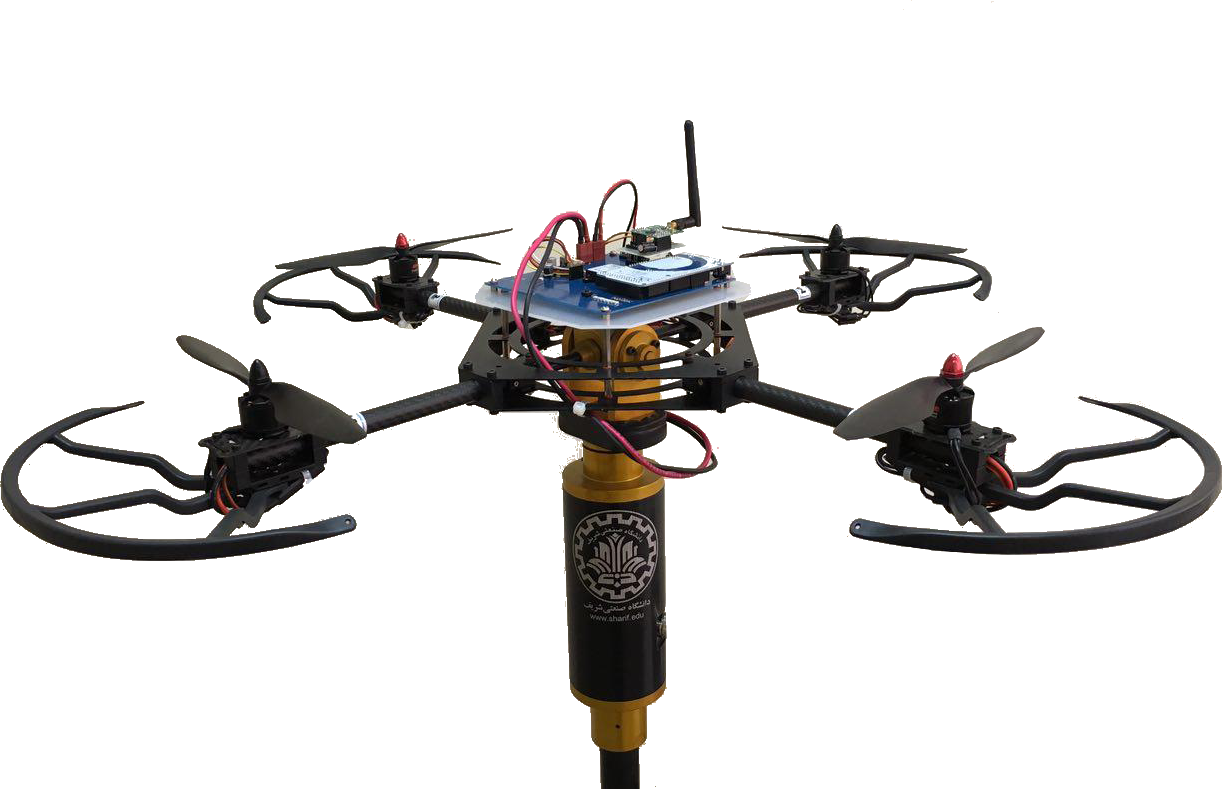
\includegraphics[width=0.7\textwidth]{../Figure/3DOFQuad.png}
   \caption{3DoF setup of the quadrotor.}
   \label{fig:quadrotor}
\end{figure}

\begin{figure}[!h]
   \centering
   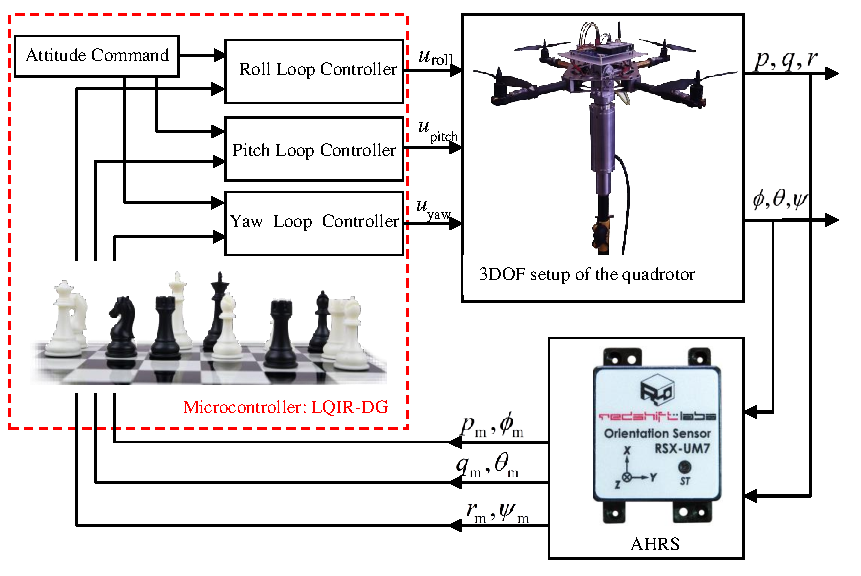
\includegraphics[width=0.7\textwidth]{../Figure/schematic.pdf}
   \caption{Block diagram of the LQIG-DG controller structure.}
   \label{fig:blockdiagram}
\end{figure}



\section{Modeling of the Quadrotor Setup}\label{sec:modeling}
Here, the model of the three-degree-of-freedom setup of the quadrotor is presented in detail. For this purpose, first, the configuration of the quadrotor is denoted. Then, the nonlinear model of the attitude dynamics is derived from denoting the state-space form. Finally, the nonlinear model is linearized to utilize for control purposes.
\subsection{Configuration of the Quadrotor}
Figure \ref{fig:schematic} denotes the quadrotor schematic. Each rotor has an angular velocity, $\Omega_r$, rotating about the $z_B$ axis in the body coordinate system. Rotors 1 and 3 rotate counterclockwise, while rotors 2 and 4 rotate clockwise to cancel yawing moment.

\begin{figure}[!h]
    \centering
    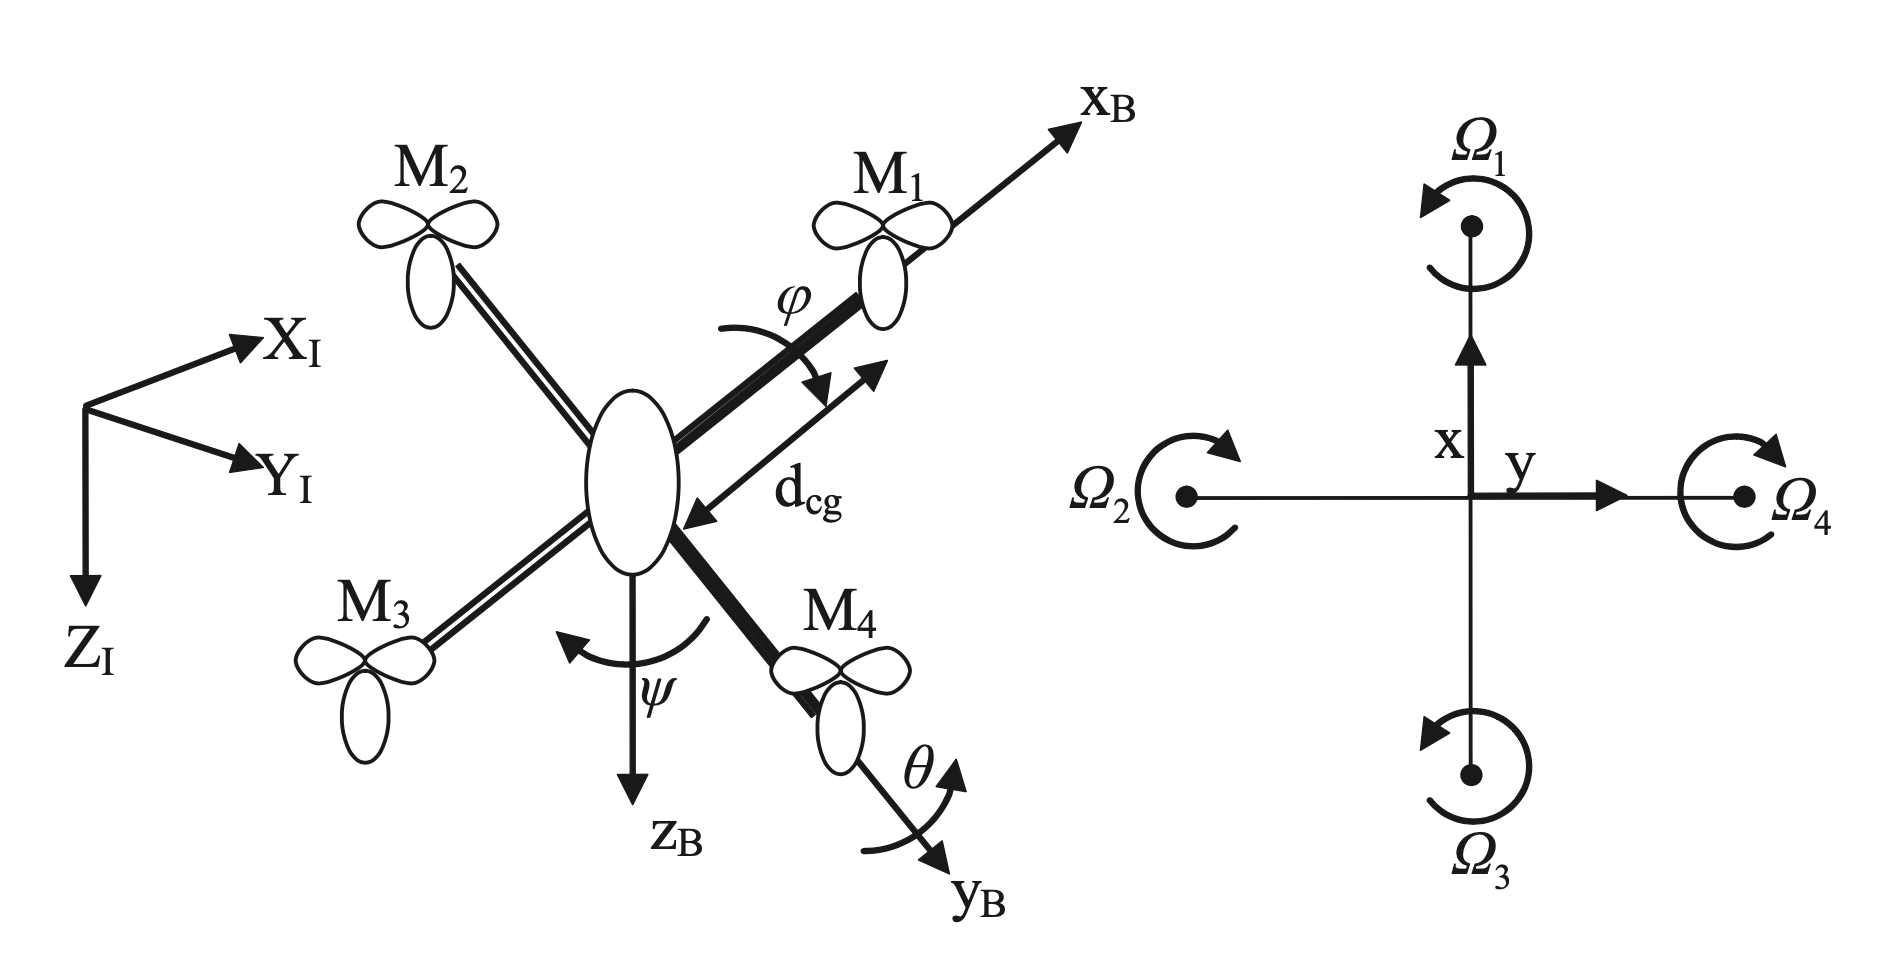
\includegraphics[width=12cm]{../Figure/schematic.png}
    \caption{Configuration of the quadrotor.}
    \label{fig:schematic}
\end{figure}

\subsection{Dynamic Model}
The quadrotor kinetic model, derived using the Newton-Euler method, is stated as \cite{4399042, article_Bouabdallah}



\begin{align}
    &\dot p = \dfrac{\mathrm{I}_{\text{yy}} - \mathrm{I}_{\text{zz}}}{\mathrm{I}_{\text{xx}}} qr + q \dfrac{\mathrm{I}_{\text{rotor}}}{\mathrm{I}_{\text{xx}}}\Omega_r + \dfrac{u_{\text{roll}}}{\mathrm{I}_{\text{xx}}} + \dfrac{d_{\text{roll}}}{\mathrm{I}_{\text{xx}}}
    \\
&\dot q = \dfrac{\mathrm{I}_{\text{zz}} - \mathrm{I}_{\text{zz}}}{\mathrm{I}_{\text{yy}}} rp + p \dfrac{\mathrm{I}_{\text{rotor}}}{\mathrm{I}_{\text{xx}}}\Omega_r + \dfrac{u_{\text{pitch}}}{\mathrm{I}_{\text{yy}}} + \dfrac{d_{\text{pitch}}}{\mathrm{I}_{\text{yy}}}
\\
&\dot r = \dfrac{\mathrm{I}_{\text{xx}} - \mathrm{I}_{\text{yy}}}{\mathrm{I}_{\text{zz}}} pq  +  \dfrac{u_{\text{yaw}}}{\mathrm{I}_{\text{zz}}} + \dfrac{d_{\text{yaw}}}{\mathrm{I}_{\text{zz}}}
\end{align}


\noindent where $(p, q, r)$ are the angular velocities. $d_{\text{roll}}$, $d_{\text{pitch}}$, and $d_{\text{yaw}}$ are the disturbances generated in $x_B$, $y_B$, and $z_B$, respectively. Moreover, $\mathrm{I}_{\text{xx}}$, $\mathrm{I}_{\text{yy}}$, and $\mathrm{I}_{\text{zz}}$ are the principal moment of inertia, and $\mathrm{I}_{\text{rotor}}$ is a rotor  inertia  about its axis.
The relation between the angular body rates and the Euler angles rates are obtained as
\begin{align}
    \dot\phi &= p + (q\sin(\phi) + r\cos(\phi))\tan(\theta)\\
\dot \theta &= q\cos(\phi) - r\sin(\phi)\\
\dot\psi &= (q\sin(\phi) + r\cos(\phi))/{\cos(\theta)}
\end{align}
where $(\phi, \theta, \psi)$ are roll, pitch, and yaw angles.
Moreover, $\Omega_r$, called the overall residual rotor angular velocity, is computed as
\begin{equation}
	\Omega_r = -\Omega_1 + \Omega_2 - \Omega_3 + \Omega_4
\end{equation}
\subsection{Control Commands}
\noindent The control inputs $u_{\text{roll}}$, $u_{\text{pitch}}$, and $u_{\text{yaw}}$ are roll, pitch, and yaw moments, obtained from the rotors, defined as
% The roll, pitch, and yaw moments produced by the propellers are the control inputs u1, u2, and u3.
\begin{align}
		&u_{\text{roll}} = \mathrm{b\,d}_{\text{cg}} (\Omega_2^2 - \Omega_4^2)\\
	&u_{\text{pitch}} = \mathrm{b\,d}_{\text{cg}} (\Omega_1^2 - \Omega_3^2) \\
	&u_{\text{yaw}} = \mathrm{d} (\Omega_1^2 - \Omega_2^2 + \Omega_3^2 - \Omega_4^2)
\end{align}

Also, d and b are, respectively, drag and thrust coefficients. $\mathrm{d}_{\text{cg}}$ is the distance of rotors from the gravity center. Hence, the angular velocity commands are obtained as
\begin{align}
		\Omega_{c, 1}^2 &= \Omega_{\text{mean}}^2 + \dfrac{1}{2\mathrm{b\,d}_{\text{cg}}}u_{\text{pitch}} + \dfrac{1}{4d}u_{\text{yaw}} \\
	\Omega_{c, 2}^2 &= \Omega_{\text{mean}}^2 + \dfrac{1}{2\mathrm{b\,d}_{\text{cg}}}u_{\text{roll}} - \dfrac{1}{4d}u_{\text{yaw}}\\
	\Omega_{c, 3}^2 &= \Omega_{\text{mean}}^2 - \dfrac{1}{2\mathrm{b\,d}_{\text{cg}}}u_{\text{pitch}} + \dfrac{1}{4d}u_{\text{yaw}} \\
\Omega_{c, 4}^2 &= \Omega_{\text{mean}}^2 - \dfrac{1}{2\mathrm{b\,d}_{\text{cg}}}u_{\text{roll}} - \dfrac{1}{4d}u_{\text{yaw}}
\end{align}
where $\Omega_{\text{mean}}$ is the nominal of the rotor angular velocities.
\subsection{State-Space Form}
\noindent Here, the state-space model is presented for control purposes.
% For control purposes, the state-space model of the quadrotor experimental setup is described.
By defining $x_1 = p$, $x_2 = q$, $x_3 = r$, $x_4 = \phi$, $x_5 = \theta$, and $x_6 = \psi$; the model of in state-space form are denoted as
% The state-space model of the experimental setup is given as
\begin{align}\label{eq:diffeq}
		\dot x_1 &= \dfrac{\mathrm{I}_{\text{yy}} - \mathrm{I}_{\text{zz}}}{\mathrm{I}_{\text{xx}}} x_2 x_3 + x_2 \dfrac{\mathrm{I}_{\text{rotor}}}{\mathrm{I}_{\text{xx}}}\Omega_r + \dfrac{u_{\text{roll}}}{\mathrm{I}_{\text{xx}}} + \dfrac{d_{\text{roll}}}{\mathrm{I}_{\text{xx}}} \\[0.5em]
	\dot x_2 &= \dfrac{\mathrm{I}_{\text{zz}} - \mathrm{I}_{\text{xx}}}{\mathrm{I}_{\text{yy}}} x_1 x_3 - x_1 \dfrac{\mathrm{I}_{\text{rotor}}}{\mathrm{I}_{\text{xx}}}\Omega_r + \dfrac{u_{\text{pitch}}}{\mathrm{I}_{\text{yy}}} + \dfrac{d_{\text{pitch}}}{\mathrm{I}_{\text{yy}}}\\[0.5em] \label{eq:diffeq-mid}
	\dot x_3 &= \dfrac{\mathrm{I}_{\text{xx}} - \mathrm{I}_{\text{yy}}}{\mathrm{I}_{\text{zz}}} x_1 x_2 + \dfrac{u_{\text{yaw}}}{\mathrm{I}_{\text{zz}}} + \dfrac{d_{\text{yaw}}}{\mathrm{I}_{\text{zz}}}\\[0.5em] 
    \dot x_4 &= x_1 + (x_2\sin(x_4) + x_3\cos(x_4))\tan(x_5)
\\[0.5em]
	\dot x_5 &= x_2\cos(x_4) - x_3\sin(x_4)\\[0.5em]
	\dot x_6 &= (x_2\sin(x_4) + x_3\cos(x_4))/\cos(x_5) \label{eq:diffeq-end}
\end{align}

Equations \eqref{eq:diffeq}-\eqref{eq:diffeq-mid} are rewritten in the following form:
\begin{align}
    \dot x_1 &= \alpha_1 x_2 x_3 + \alpha_2 x_2\Omega_r + \alpha_3 u_{\text{roll}} + \alpha_3 d_{\text{roll}} \\[0.5em]
\dot x_2 &= \beta_1 x_1 x_3 - \beta_2 x_1\Omega_r + \beta_3 u_{\text{pitch}}+ \beta_3 d_{\text{pitch}}\\[0.5em]
\dot x_3 &= \gamma_1 x_1 x_2 + \gamma_2u_{\text{yaw}} + \gamma_2d_{\text{yaw}}
\end{align}

The measurement model is written as
\begin{equation}
	\begin{split}
		\boldsymbol{\mathrm{z}} &= \begin{bmatrix}
			p_m & q_m & r_m & \phi_m & \theta_m & \psi_m
		\end{bmatrix}^\mathrm{T}
	\end{split}
\end{equation}
\subsection{Linear Model}
\noindent The continuous-time linear model is utilized to drive the control commands on the quadrotor. The linear state-space model is denoted as
\begin{equation}\label{eq:linear}
	\boldsymbol{\dot{\mathrm{x}}}(t) = \boldsymbol{\mathrm{Ax}}(t) + \boldsymbol{\mathrm{Bu}}(t) + \boldsymbol{\mathrm{B_{d}d}}(t)
\end{equation}
where $\boldsymbol{\mathrm{A}}$, $\boldsymbol{\mathrm{B}}$, and $\boldsymbol{\mathrm{B_d}}$ are the system, input and disturbance matrices, respectively. Moreover, $\boldsymbol{\mathrm{d}}$ is the disturbance. The measurements equation is stated as
\begin{equation}
	\boldsymbol{{\mathrm{z}}}(t) = \boldsymbol{\mathrm{x}}(t)
\end{equation}
According to equations\eqref{eq:diffeq}-\eqref{eq:diffeq-end}, the linear dynamic model around the equilibrium points $(\boldsymbol{{\mathrm{x}}}_e\!=\!0 \text{ and } \boldsymbol{{\mathrm{u}}}_e\!=\!0)$ of the quadrotor setup is denoted as
\begin{equation}
	\begin{split}
		\boldsymbol{{\mathrm{\dot x}}} = \begin{bmatrix}
			\boldsymbol{{\mathrm{\dot x_{\text{roll}}}}}\\
			\boldsymbol{{\mathrm{\dot x_{\text{pitch}}}}}\\
			\boldsymbol{{\mathrm{\dot x_{\text{yaw}}}}}
		\end{bmatrix} &= \begin{bmatrix}
			\boldsymbol{{\mathrm{A_{\text{roll}}}}} & \boldsymbol{0} & \boldsymbol{0}\\
			\boldsymbol{0} & \boldsymbol{{\mathrm{A_{\text{pitch}}}}} & \boldsymbol{0} \\
			\boldsymbol{0} & \boldsymbol{0} & \boldsymbol{{\mathrm{A_{\text{yaw}}}}}
		\end{bmatrix} \begin{bmatrix}
			\boldsymbol{{\mathrm{x_{\text{roll}}}}}\\
			\boldsymbol{{\mathrm{x_{\text{pitch}}}}}\\
			\boldsymbol{{\mathrm{x_{\text{yaw}}}}}
		\end{bmatrix}
		\\[1em]
		& + \begin{bmatrix}
			\boldsymbol{{\mathrm{B_{\text{roll}}}}} & \boldsymbol{0} & \boldsymbol{0}\\
			\boldsymbol{0} & \boldsymbol{{\mathrm{B_{\text{pitch}}}}} & \boldsymbol{0} \\
			\boldsymbol{0} & \boldsymbol{0} & \boldsymbol{{\mathrm{B_{\text{yaw}}}}}
		\end{bmatrix}
		\begin{bmatrix}
			\boldsymbol{{\mathrm{u_{\text{roll}}}}}\\
			\boldsymbol{{\mathrm{u_{\text{pitch}}}}}\\
			\boldsymbol{{\mathrm{u_{\text{yaw}}}}}
		\end{bmatrix}\\[1em]
		& + \begin{bmatrix}
			\boldsymbol{{\mathrm{B_{\text{roll}}}}} & \boldsymbol{0} & \boldsymbol{0}\\
			\boldsymbol{0} & \boldsymbol{{\mathrm{B_{\text{pitch}}}}} & \boldsymbol{0} \\
			\boldsymbol{0} & \boldsymbol{0} & \boldsymbol{{\mathrm{B_{\text{yaw}}}}}
		\end{bmatrix} \begin{bmatrix}
			\boldsymbol{{\mathrm{d_{\text{roll}}}}}\\
			\boldsymbol{{\mathrm{d_{\text{pitch}}}}}\\
			\boldsymbol{{\mathrm{d_{\text{yaw}}}}}
		\end{bmatrix}
	\end{split}
\end{equation}
where $\boldsymbol{\mathrm{x}}_{\text{roll}} = \begin{bmatrix}
	p & \phi
\end{bmatrix}^\mathrm{T}$, $\boldsymbol{\mathrm{x}}_{\text{pitch}} = \begin{bmatrix}
	q & \theta \end{bmatrix}^\mathrm{T}$, and $\boldsymbol{\mathrm{x}}_{\text{yaw}} = \begin{bmatrix}
	r & \psi
\end{bmatrix}^\mathrm{T}$.



Moreover, the state and input matrices are presented as
\begin{equation}
	\begin{split}
		\boldsymbol{\mathrm{A}}_{\text{roll}}  =\boldsymbol{\mathrm{A}}_{\text{pitch}}  = \boldsymbol{\mathrm{A}}_{\text{yaw}}  = \begin{bmatrix}
			0 & 0\\
			1 & 0
		\end{bmatrix}
	\end{split}
\end{equation}

\begin{equation}
	\begin{split}
		\boldsymbol{\mathrm{B}}_{\text{roll}}  = \begin{bmatrix}
			\dfrac{1}{\mathrm{I}_{\text{xx}}}
			\\[1em]
			0
		\end{bmatrix};~ \boldsymbol{\mathrm{B}}_{\text{pitch}}  = \begin{bmatrix}
			\dfrac{1}{\mathrm{I}_{\text{yy}}}
			\\[1em]
			0
		\end{bmatrix};~ \boldsymbol{\mathrm{B}}_{\text{yaw}}  = \begin{bmatrix}
			\dfrac{1}{\mathrm{I}_{\text{zz}}}
			\\[1em]
			0
		\end{bmatrix}
	\end{split}
\end{equation}

\subsection{System Identification}

\noindent Here, the system identification was made using the simulation of the roll, pitch, and yaw states and sensor data output from the quadrotor setup. For this purpose, the same input is given to the simulated model and setup. In the case of system identification, the cost function was defined as the sum square error between simulations and quadrotor setup measurements. Then, the Nonlinear Least Squares (NLS)  optimization technique minimizes the cost function. In NLS, the goal is to look for the model parameters vector $
\rho = \begin{bmatrix}
    \alpha_1 & \alpha_2 & \alpha_3 & \beta_1 & \beta_2 & \beta_3 & \gamma_1 & \gamma_2
\end{bmatrix}
$, which would minimize the sum of squares of residual errors. In other words, the following cost function has to minimize:

\begin{equation}
    \text{Residual sum of squares} = RSS = \sum_{i=1}^{n} \left(y_i - \hat y_i \right)^2
\end{equation}
where $y$ is the value of the variable to be predicted, and $ \hat y$ is the predicted value of  $y$, which $\hat y$ is a function of the 3DoF setup model parameters vector, $\rho$,  and the system states, $\boldsymbol{{\mathrm{x}}}$, i.e.:
\begin{equation}
    \hat y_i = f(\boldsymbol{{\mathrm{x}}}_i, \rho)
\end{equation}
One way to minimize RSS is to differentiate RSS with respect to $\rho$, then set the differentiation to zero and solve for  $\rho$,  i.e.:
\begin{equation}
    \dfrac{\partial }{\partial \rho_j} RSS = 0, \quad \forall j \in [1, n]
\end{equation}
Since there is no closed-form solution for this system of equations, so iterative optimization technique has to be used in which, at each iteration k, minor adjustments have been made to the values of  $\rho$ as shown below, and re-evaluate RSS:
\begin{equation}
    \rho_j^{(k)} = \rho_j^{(k-1)} + \delta \rho_j
\end{equation}
Trust Region Reflective (TRR) has been devised to update $\rho$ efficiently. To increase the accuracy of system identification, at first, the parameters of each channel were estimated separately, and then the coupled parameters of the attitude channels were modified. In the parameter modification process, after each parameter modification step mentioned above, the estimated parameters of the previous step are assumed to be fixed, and other parameters are modified. To identification of each stage, several experiments with different scenarios have been performed.

\section{Formulation of the Controller Design}\label{sec:controller}
\noindent In the LQIR-DG controller structure, an integral action is added to the LQR-DG controller to cancel the steady-state errors for reference tracking. For this purpose, first, the augmented state space of the linear quadrotor model is defined to utilize in the controller architecture. Then, the LQR-DG controller design procedure is presented to produce the best control commands for the experimental setup of the quadrotor.

\subsection{Augmented State Space Formulation}
\noindent To add the integral action to the controller structure, the augmented states are defined as follows:
\begin{equation}\label{lqidg_x}
    \boldsymbol{\mathrm{x_{a_i}}} = \begin{bmatrix}
        \boldsymbol{\mathrm{x_i}} &
        \displaystyle \int \boldsymbol{\mathrm{x_i}}
    \end{bmatrix}^\mathrm{T}
\end{equation}
where $i$ = roll, pitch, and yaw.
Then, the quadrotor dynamics model, denoted by Eq.\eqref{eq:linear}, is denoted in the augmented state-space model as

\begin{equation}\label{systemlqidg}
	\begin{split}
		\boldsymbol{\dot{\mathrm{x}}_a}(t) &= \boldsymbol{\mathrm{A_ax_a}}(t) + \boldsymbol{\mathrm{B_{{a}}u}}(t) + \boldsymbol{\mathrm{B_{{d_a}}d}}(t)%, \quad \boldsymbol{x}(0) = 
	\end{split}
\end{equation}
where matrices $\boldsymbol{\mathrm{A_a}}$ and $\boldsymbol{\mathrm{B_a}}$ are defined as follows:

\begin{equation}
	\boldsymbol{\mathrm{A_a}} = \begin{bmatrix}
		\boldsymbol{\mathrm{A}} & \boldsymbol{0}\\
		\boldsymbol{\mathrm{I}} & \boldsymbol{0}
	\end{bmatrix}
\end{equation}
\begin{equation}
	\boldsymbol{\mathrm{B_a}} = \boldsymbol{\mathrm{B_{{d_a}}}} = \begin{bmatrix}
		\boldsymbol{\mathrm{B}}\\
		\boldsymbol{0}
	\end{bmatrix}
\end{equation}
In the above equation $\boldsymbol{\mathrm{I}}$ denotes the identity matrix.

\subsection{LQIR-DG Controller Method}
\noindent The LQIR-DG controller is an optimal and robust method based on the differential game theory. This controller consists of two essential players: one finds the best control command, and the other creates the worst disturbance. 
For this purpose, the first player tries to minimize a cost function, while the second is assumed to maximize it. Therefore, the quadratic cost function equation is denoted using min-max operators as follows:
\begin{equation}
    \min_{u} \max_{d} J(\boldsymbol{\mathrm{x_{a_i}}}, {u_i}, {d_i}) = J(\boldsymbol{\mathrm{x_{a_i}}}, {u^*_i}, {d^*_i})=\min_{u} \max_{d}
     \int_{0}^{\mathrm{t_f}}\biggl (\boldsymbol{\mathrm{x^\mathrm{T}_{a_i}}}  \boldsymbol{\mathrm{Q_i}} \boldsymbol{\mathrm{x_{a_i}}}+
    {{u^\mathrm{T}_i}}  {{R}} {{u_i}}-
    {{d^\mathrm{T}_{i}}} {{ R_{d} d_{i}}}
    \biggl )\mathrm{d}t
\end{equation}
where ${{ R}}$ and ${{R_{d}}}$ are symmetric nonnegative definite matrices and $\boldsymbol{\mathrm{Q_i}} $ is a symmetric positive definite matrix.  Moreover, $\mathrm{t_f}$ is the final time. ???????????????????To solve this problem, connections between the general optimal problem and the LQIR problem are considered \cite{LQDG}. Consequently, the optimum control effort is computed for each control loop as follows:

\begin{align}
		{{u_i}}(t) &= -\boldsymbol{{\mathrm{K}}_{i}}(t) \boldsymbol{{\mathrm{x_{a_i}}}}(t)\\
	{{d_i}}(t) &=\boldsymbol{{\mathrm{K_{d_i}}}}(t)\boldsymbol{{\mathrm{x_{a_i}}}}(t)
\end{align}
where $\boldsymbol{{\mathrm{K_i}}}$ and $\boldsymbol{{\mathrm{K_{d_i}}}}$ are a time varying gain, given by
\begin{align}
	\boldsymbol{{\mathrm{K_i}}} &= {{{R}}^{-1}}\boldsymbol{{\mathrm{B}_{a_i}^\mathrm{T}}}\boldsymbol{{\mathrm{P}}_{a_i}}(t)\\
	\boldsymbol{{\mathrm{K_{d_i}}}} &= {{{R}}^{-1}_{d}}\boldsymbol{{\mathrm{B}_{a_{d_i}}^\mathrm{T}}}\boldsymbol{{\mathrm{P}}_{a_{d_i}}}(t)
\end{align}
where $\boldsymbol{{\mathrm{P}}_{a_i}}(t)$ and $\boldsymbol{{\mathrm{P}}_{a_{d_i}}}(t)$ satisfy
\begin{align}\label{coupled_riccatti_LQIDG}
            \boldsymbol{\dot{\mathrm{P}}_{a_i}}(t) &= -\boldsymbol{\mathrm{A^\mathrm{T}_a}}\boldsymbol{\mathrm{P_{a_i}}}(t) - \boldsymbol{\mathrm{P_{a_i}}}(t)\boldsymbol{\mathrm{A_a}} - \boldsymbol{\mathrm{Q_i}} +\boldsymbol{\mathrm{P_{a_i}}}(t)\boldsymbol{\mathrm{S_{a_i}}}(t)\boldsymbol{\mathrm{P_{a_i}}}(t) + \boldsymbol{\mathrm{P_{a_i}}}(t)\boldsymbol{\mathrm{S_{a_{d_i}}}}(t)\boldsymbol{\mathrm{P_{a_{d_i}}}}(t)\\
            \boldsymbol{\dot{\mathrm{P}}_{a_{d_i}}}(t) &= -\boldsymbol{\mathrm{A^\mathrm{T}_a}}\boldsymbol{\mathrm{P_{a_{d_i}}}}(t) - \boldsymbol{\mathrm{P_{a_{d_i}}}}(t)\boldsymbol{\mathrm{A_a}} - \boldsymbol{\mathrm{Q_{i}}} +\boldsymbol{\mathrm{P_{a_{d_i}}}}(t)\boldsymbol{\mathrm{S_{a_{d_i}}}}(t)\boldsymbol{\mathrm{P_{a_{d_i}}}}(t) + \boldsymbol{\mathrm{P_{a_{d_i}}}}(t)\boldsymbol{\mathrm{S_{a_i}}}(t)\boldsymbol{\mathrm{P_{a_i}}}(t)
\end{align}
where $\boldsymbol{\mathrm{S_{a_i}}} = \boldsymbol{\mathrm{B_{a_i}}}R^{-1}\boldsymbol{\mathrm{B}^\mathrm{T}_{a_i}}$ and $\boldsymbol{\mathrm{S_{a_{d_i}}}} = \boldsymbol{\mathrm{B}_{a_{d_i}}}R_{d}^{-1}\boldsymbol{\mathrm{B}^\mathrm{T}_{a_{d_i}}}$.
In this study, the steady-state values of the above equations $(\boldsymbol{{\mathrm{P}}} \text{ as } \mathrm{t_f} \to \infty)$ are utilized to generate a feedback control law.

\section{Result and Discussion}\label{sec:results}\label{sec:results}


\noindent Here, the results of the LQIR-DG controller method are devoted to the control loops of the roll, pitch, and yaw of the experimental setup of the quadrotor. First, the controller parameters are tuned using the results of numerical simulations. Moreover, the performance of the LQIR-DG controller is compared to an LQR control strategy. The quadrotor parameters are shown in table \ref{tab:parameters}.
% Table I provides the quadrotor's characteristics.
Moreover, the parameters of LQIR-DG controller weight are denoted in table \ref{tab:control weight_new}.
\begin{table}[!h]
	\renewcommand{\arraystretch}{1.3}
	\caption{The Parameter of the Quadrotor}
	\begin{center}
	\begin{tabular}{c c c}
	\hline
	\textbf{Parameter} & \textbf{\textit{Value}}& \textbf{\textit{Unit}} \\
	\hline
	$\mathrm{I}_{\text{xx}}$ & $0.02839$ & $\mathrm{kg.m^2}$ \\
	$\mathrm{I}_{\text{yy}}$  & $0.03066$ & $\mathrm{kg.m^2}$\\
	$\mathrm{I}_{\text{zz}}$  & $0.0439$ & $\mathrm{kg.m^2}$ \\
	$\mathrm{I}_{\text{rotor}}$  & $4.4398\times 10^{-5}$ & $\mathrm{kg.m^2}$\\
	$\mathrm{b}$  & $3.13\times10^{-5}$ & $\mathrm{N.\sec^2/rad^2}$ \\
	$\mathrm{d}$  & $3.2\times10^{-6}$ & $\mathrm{N.m.\sec^2/rad^2}$\\
	$\Omega_{\text{mean}}$ & $3000$ & $\mathrm{rpm}$\\
	$\mathrm{d}_{\text{cg}}$  & $0.2$ & $\mathrm{m}$\\
	\hline
	\end{tabular}
	\label{tab:parameters}
	\end{center}
\end{table}


\begin{table}[!h]
	\renewcommand{\arraystretch}{1.3}
	\caption{The Parameters of the LQIR-DG Controller?????????????}
	\begin{center}
	\begin{tabular}{c c c}
	\hline
	\textbf{Control Loop} & \textbf{\textit{Weight}}& \textbf{\textit{Value}} \\
	\hline
	Roll & 
	$\boldsymbol{{\mathrm{Q_{\text{roll}}}}}$ & diag([$7.91$, $0.01$, $631.85$, $214.28$])\\
	Pitch & 
	$\boldsymbol{{\mathrm{Q_{\text{pitch}}}}}$ & diag([$9853.09$, $0.12$, $0.01$, $873.93$])\\
	Yaw & 
	$\boldsymbol{{\mathrm{Q_{\text{yaw}}}}}$ & diag([$1.81e\!-\!4$, $4.5e\!-\!4$, $3e\!-\!6$, $1.7e\!-\!5$])\\
	-& $R$ & 1\\
	-& $R_{d}$ & 1.2577\\
	% $4.5e\!-\!5$])\\
	%  & 
	%  \\
	% Yaw & 
	% $3e\!-\!6$ & $1.7e\!-\!5$ & $1.81e\!-\!4$ &
	% $4.5e\!-\!5$ \\
	\hline
	\end{tabular}
	\end{center}
	\label{tab:control weight_new}
\end{table}




\subsection{Evaluation of the 3DoF experimental setup model}

\noindent Here, the performance of the extracted model of the 3DoF experimental setup is evaluated un-der three scenarios: (i) each channel separately, (ii) coupling between roll and pitch channel, and (iii) coupling between roll, pitch, and yaw channel. In the first scenario, each channel's parame-ters are changed.
%  The results of the first scenario are shown in figure \ref{fig:3dof model}. The results of the second scenario are shown in figure \ref{fig:3dof model2}. The results of the third scenario are shown in figure \ref{fig:3dof model3}


\begin{minipage}[t]{0.95\linewidth}
	\hfill
    \begin{minipage}[b]{0.48\linewidth}
		\centering
		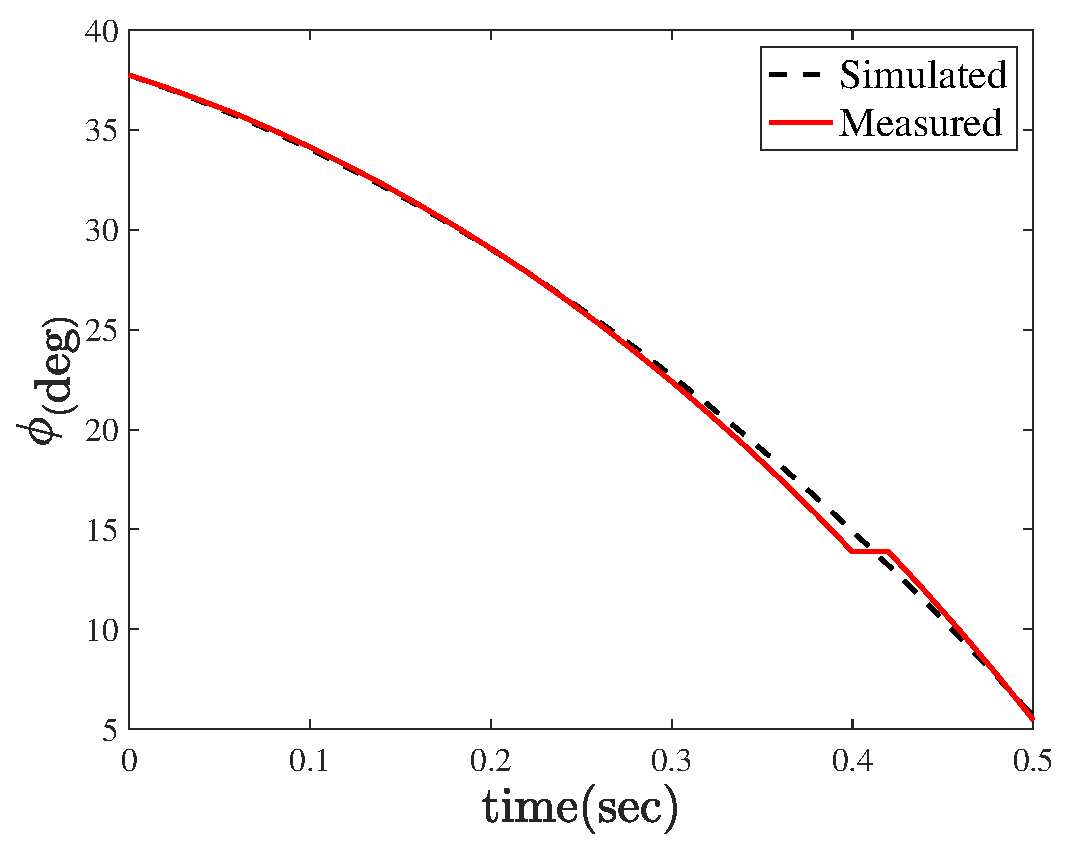
\includegraphics[width=1\linewidth]{../Figure/parameter_estimation/roll/roll}
		\captionsetup{justification=centering}
		\captionof{figure}{Comparison of roll channel states in simulation and 3DoF setup}
	\end{minipage}
	\begin{minipage}[b]{0.49\linewidth}
		\centering
		\begin{tabular}{ccc}\hline
			Parameter & Value & Value after evaluation
            \Tstrut\\ \hline
			$\alpha_3$  & $1.1\times10^{-4}$ & $5.47\times10^{-5}$  \Tstrut\\ \hline
			\\
			\\\\\\\\\\\\\\\\\\
		\end{tabular}
	\captionsetup{justification=centering}
		\captionof{table}{Comparison of roll channel parameter values before and after evaluation}
	\end{minipage}
    \vspace{1cm}
\end{minipage}






\begin{minipage}[t]{0.95\linewidth}
	\hfill
    \begin{minipage}[b]{0.48\linewidth}
		\centering
		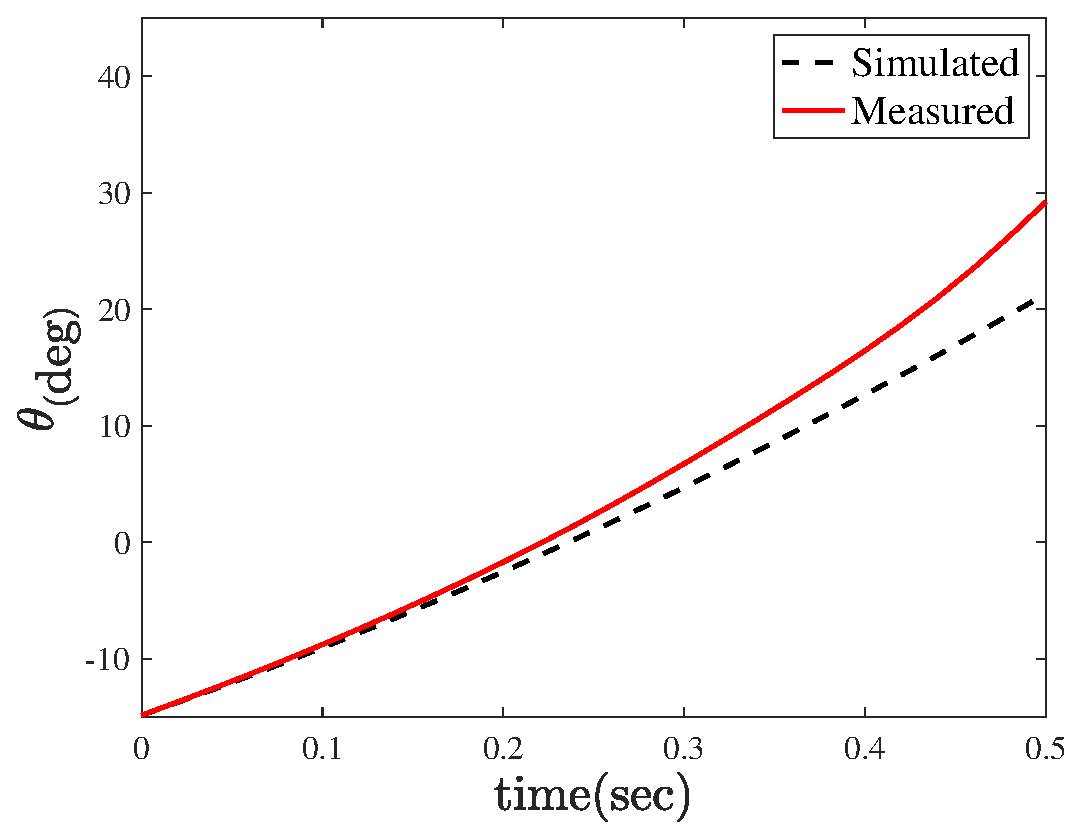
\includegraphics[width=1\linewidth]{../Figure/parameter_estimation/pitch/pitch}
		\captionsetup{justification=centering}
		\captionof{figure}{Comparison of pitch channel states in simulation and 3DoF setup}
	\end{minipage}
	\begin{minipage}[b]{0.49\linewidth}
		\centering
		\begin{tabular}{ccc}\hline
			Parameter & Value & Value after evaluation
            \Tstrut\\ \hline
			$\beta_3$  & $1.1\times10^{-4}$ & $7.13\times10^{-5}$  \Tstrut\\ \hline
			\\
			\\\\\\\\\\\\\\\\\\
		\end{tabular}
	\captionsetup{justification=centering}
		\captionof{table}{Comparison of pitch channel parameter values before and after evaluation}
	\end{minipage}
\end{minipage}

% \vspace{1cm}

\begin{minipage}[t]{0.95\linewidth}
	\hfill
    \begin{minipage}[b]{0.48\linewidth}
		\centering
		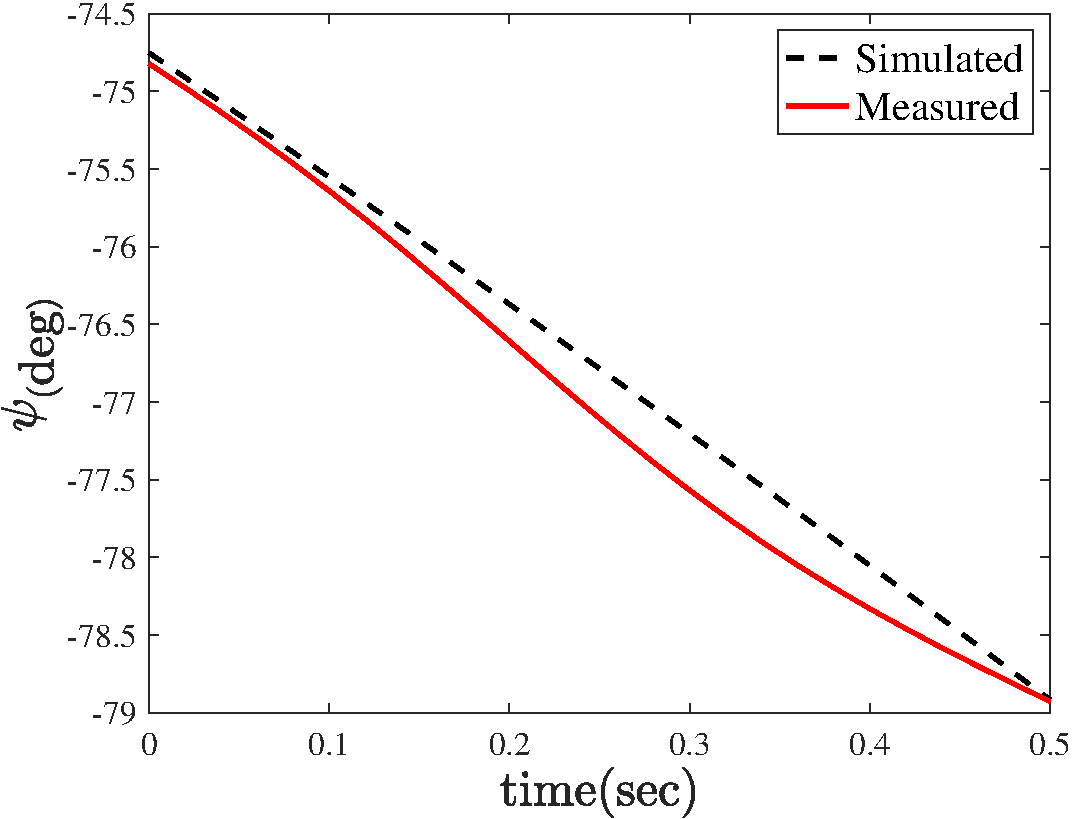
\includegraphics[width=1\linewidth]{../Figure/parameter_estimation/yaw/yaw}
		\captionsetup{justification=centering}
		\captionof{figure}{Comparison of yaw channel states in simulation and 3DoF setup}
	\end{minipage}
	\begin{minipage}[b]{0.49\linewidth}
		\centering
		\begin{tabular}{ccc}\hline
			Parameter & Value & Value after evaluation
            \Tstrut\\ \hline
			$\gamma_2$  & $5.5\times10^{-5}$ & $1.3\times10^{-6}$  \Tstrut\\ \hline
			\\
			\\\\\\\\\\\\\\\\\\
		\end{tabular}
	\captionsetup{justification=centering}
		\captionof{table}{Comparison of yaw channel parameter values before and after evaluation}
	\end{minipage}
\end{minipage}

\begin{minipage}[t]{0.95\linewidth}
	\hfill
    \begin{minipage}[b]{0.48\linewidth}
		\centering
		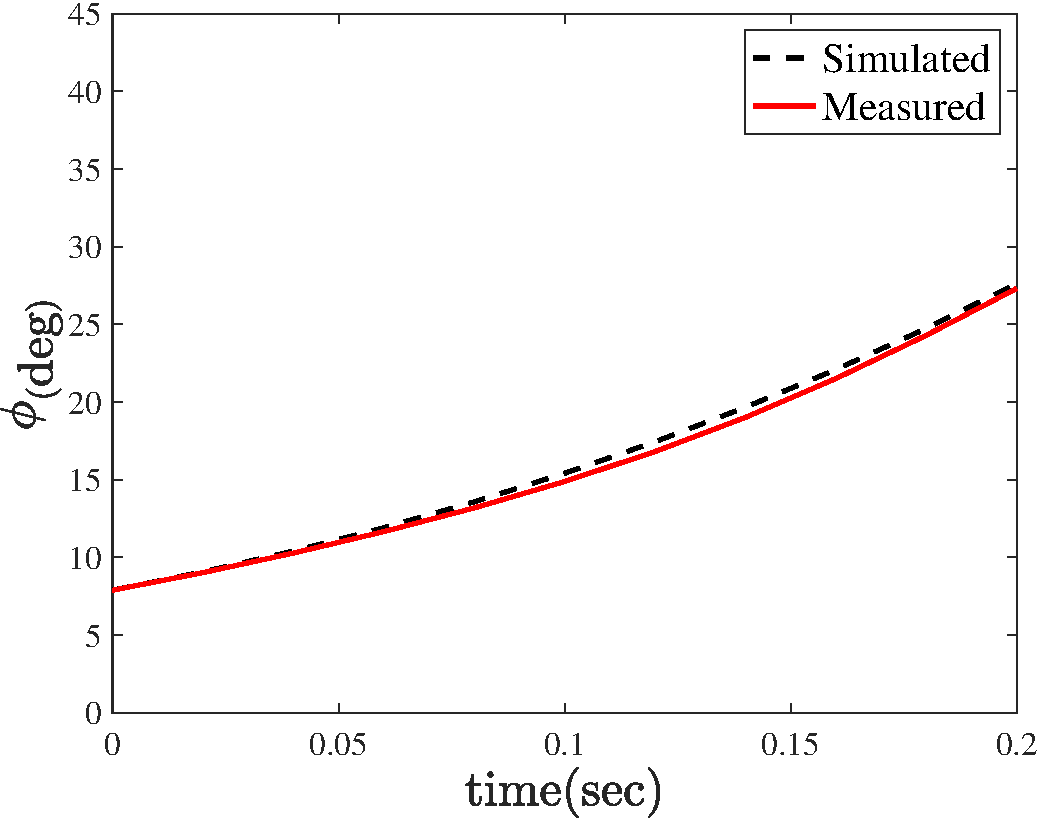
\includegraphics[width=1\linewidth]{../Figure/parameter_estimation/roll-pitch/roll}
		\captionsetup{justification=centering}
		\captionof{figure}{Comparison of roll channel states in simulation and 3DoF setup}
	\end{minipage}
    \begin{minipage}[b]{0.48\linewidth}
		\centering
		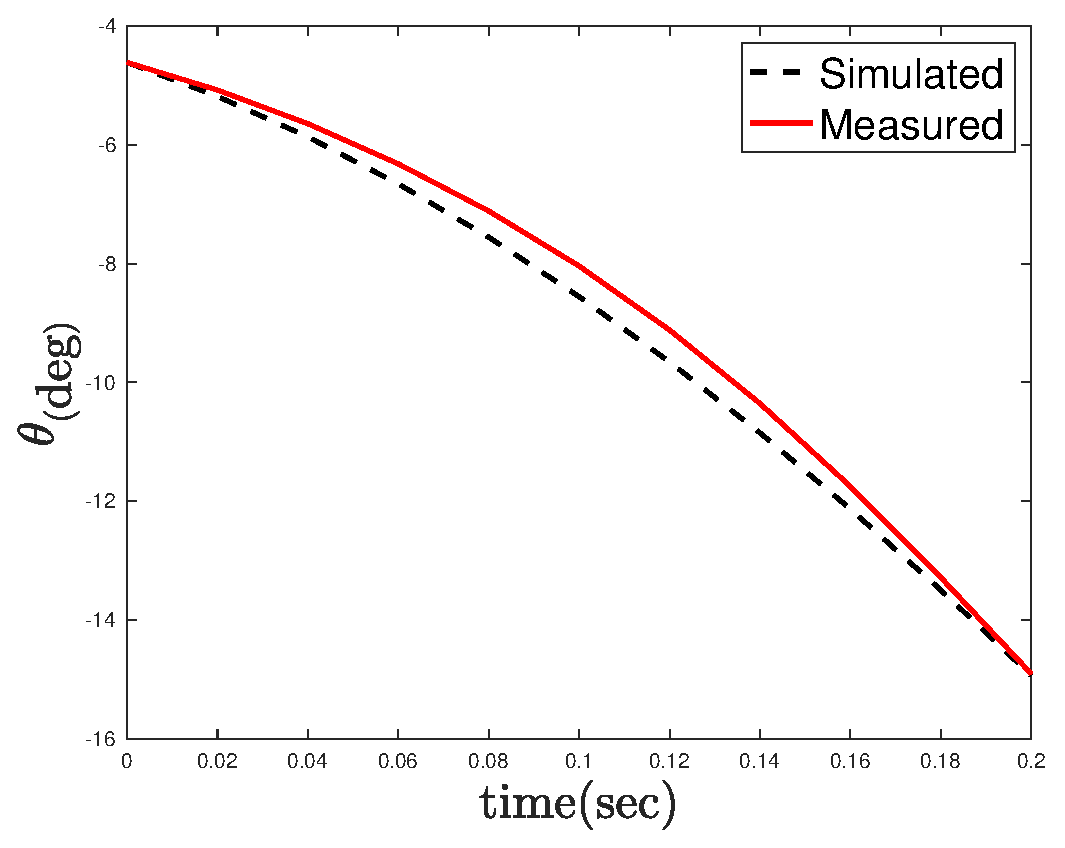
\includegraphics[width=1\linewidth]{../Figure/parameter_estimation/roll-pitch/pitch}
		\captionsetup{justification=centering}
		\captionof{figure}{Comparison of pitch channel states in simulation and 3DoF setup}
	\end{minipage}
    \hfill
    \begin{minipage}[b]{1\linewidth}
		\centering
		\begin{tabular}{ccc}\hline
			Parameter & Value & Value after evaluation
            \Tstrut\\ \hline
			$\alpha_2$  & 0.0015 & 0.0020\Tstrut\\
            $\beta_2$  & 0.0015 & 0.0027\Tstrut\\ \hline
		\end{tabular}
	\captionsetup{justification=centering}
		\captionof{table}{Comparison of roll-pitch channel parameter values before and after evaluation}
	\end{minipage}
\end{minipage}


    \begin{minipage}[b]{0.48\linewidth}
		\centering
		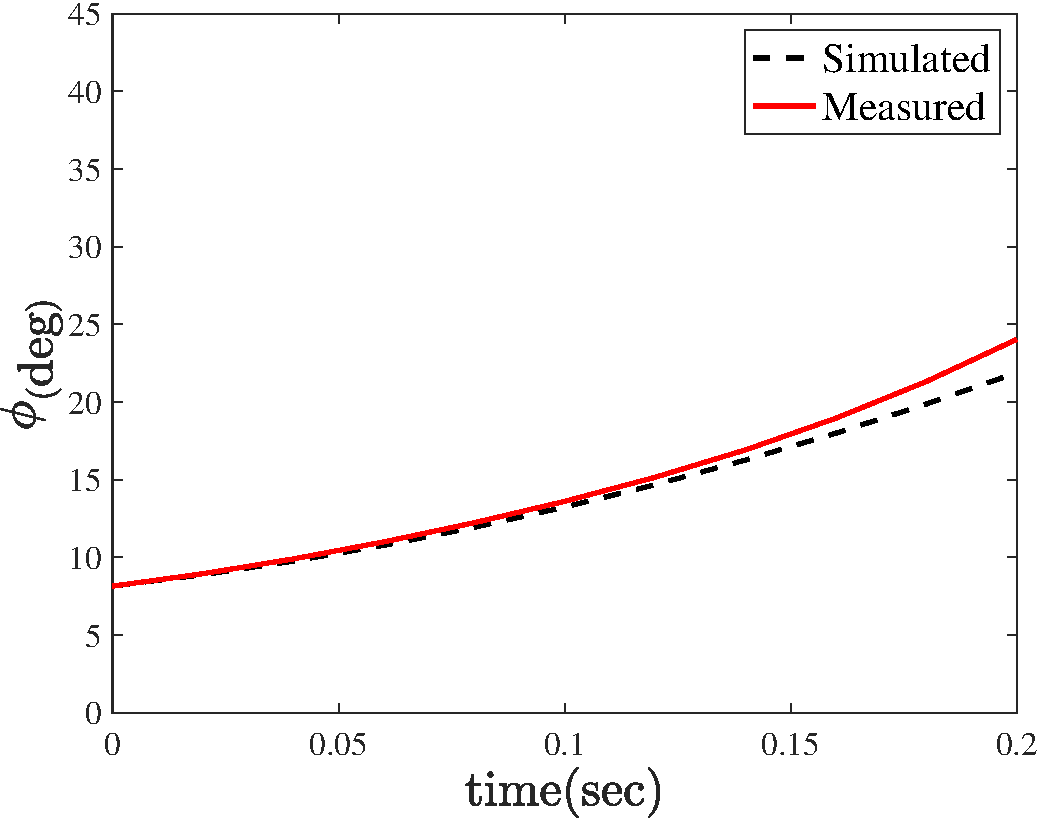
\includegraphics[width=1\linewidth]{../Figure/parameter_estimation/3DOF/roll}
		\captionsetup{justification=centering}
		\captionof{figure}{Comparison of roll channel states in simulation and 3DoF setup}
	\end{minipage}
    \begin{minipage}[b]{0.48\linewidth}
		\centering
		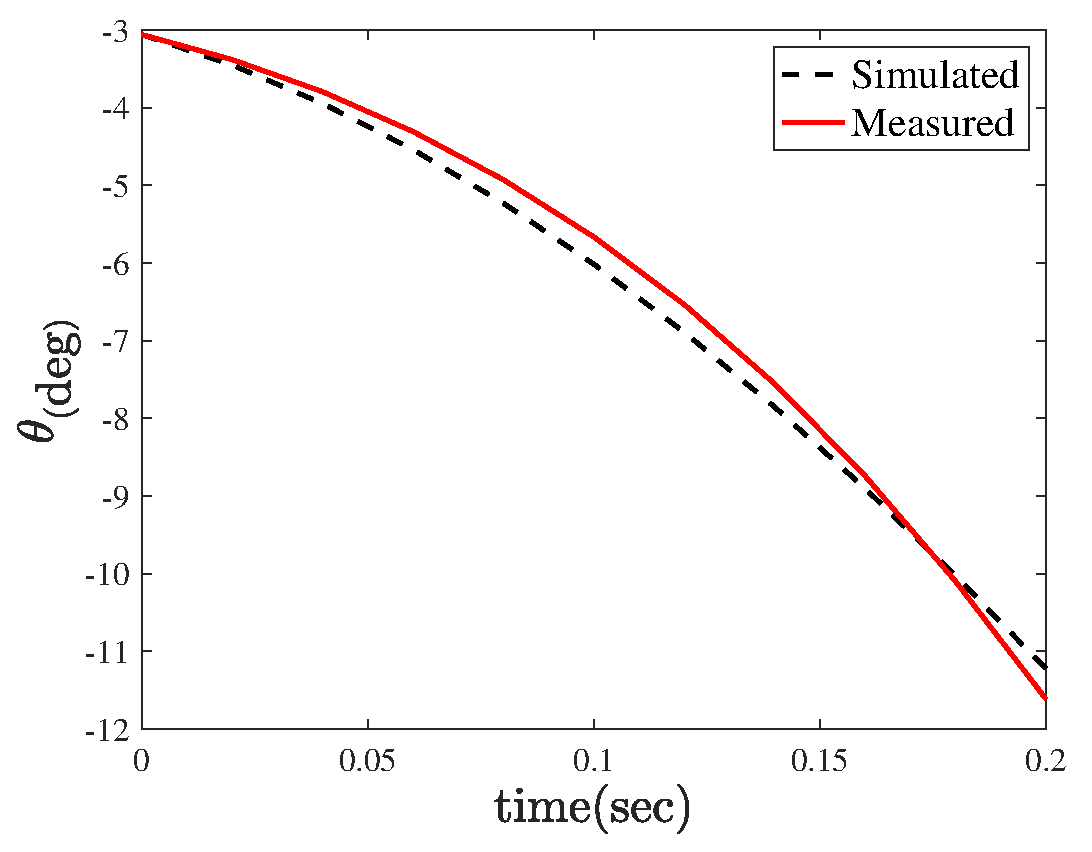
\includegraphics[width=1\linewidth]{../Figure/parameter_estimation/3DOF/pitch}
		\captionsetup{justification=centering}
		\captionof{figure}{Comparison of pitch channel states in simulation and 3DoF setup}
	\end{minipage}
    \hfill
    \begin{minipage}[b]{0.48\linewidth}
		\centering
		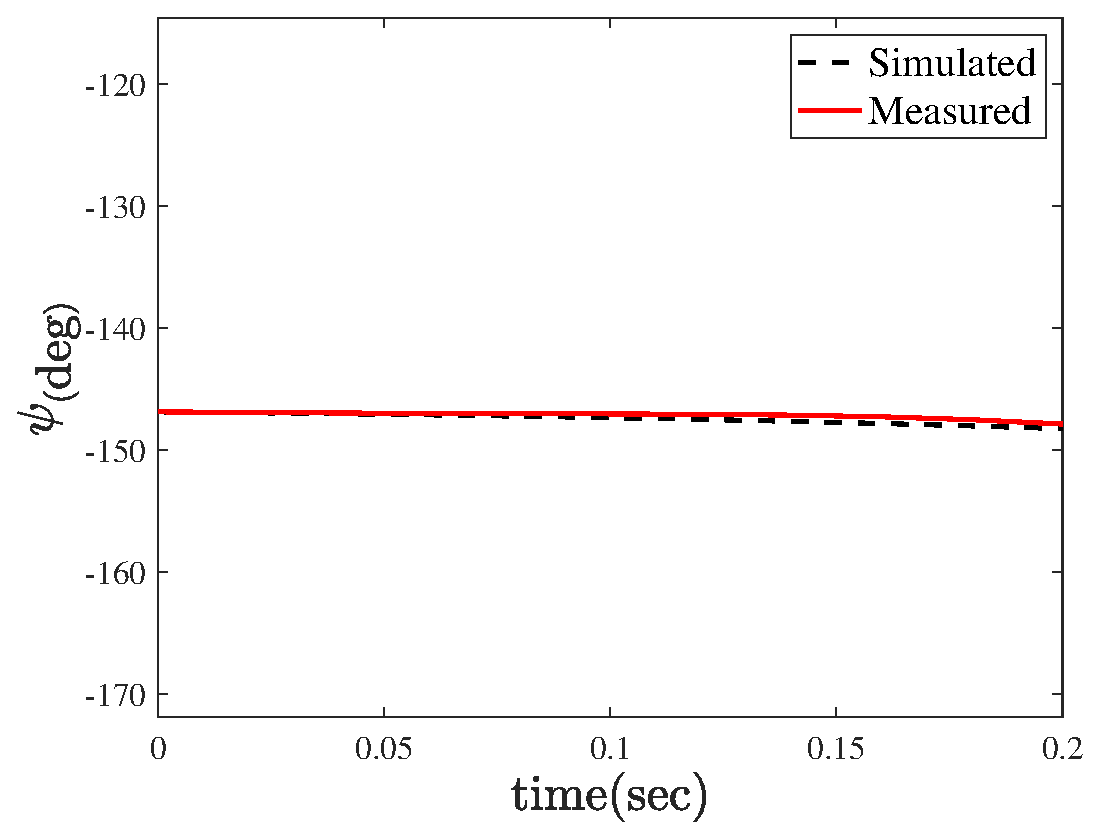
\includegraphics[width=1\linewidth]{../Figure/parameter_estimation/3DOF/yaw}
		\captionsetup{justification=centering}
		\captionof{figure}{Comparison of yaw channel states in simulation and 3DoF setup}
	\end{minipage}
    \begin{minipage}[b]{0.48\linewidth}
		\centering
		\begin{tabular}{ccc}\hline
			Parameter & Value & Value after evaluation
            \Tstrut\\ \hline
			$\alpha_1$  & -0.9628 & -1.56\Tstrut\\
            $\beta_1$  & 0.9629 & 1.57\Tstrut \\
            $\gamma_1$  & -0.0017 &-0.085\Tstrut\\ \hline
            \\\\\\\\\\\\\\\\
		\end{tabular}
	\captionsetup{justification=centering}
		\captionof{table}{Comparison of 3DOF channel parameter values before and after evaluation}
	\end{minipage}


\subsection{Performance of the LQIR-DG Controller}
\noindent Here, the performance of the LQIR-DG controller is evaluated. The desired and actual outputs, including the roll, pitch, and yaw angles, are compared in figure \ref{fig:result}. The desired scenario of the simulator is considered a level flight. These figures show that the attitude outputs of the quadrotor converge to the desired values in less than three seconds. Moreover, figure \ref{fig:omega} shows the angular velocity command of the quadrotor, 
respectively. These results illustrate that the LQIR-DG approach appropriately controls the attitude of the experimental setup of the quadrotor.


\begin{figure}[!h]
	\centering
	\subfloat[]{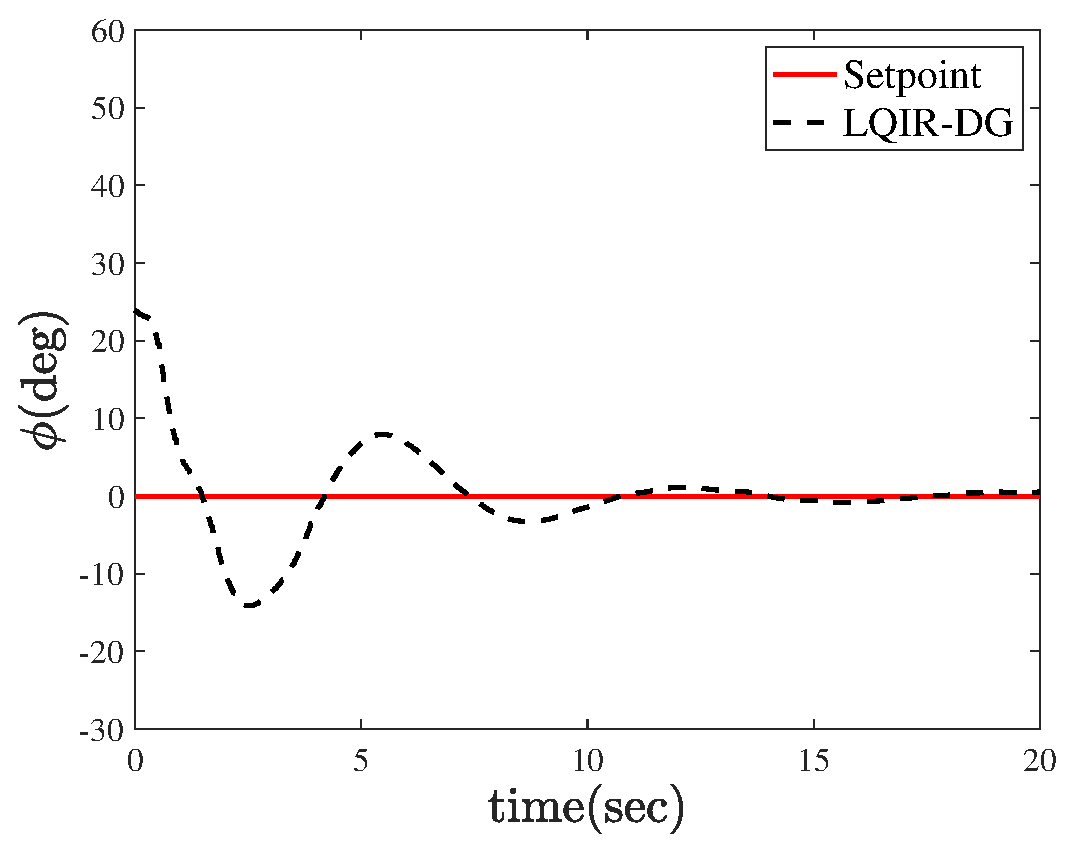
\includegraphics[width=.49\linewidth]{../Figure/implementation/lqidg_roll}}\subfloat[]{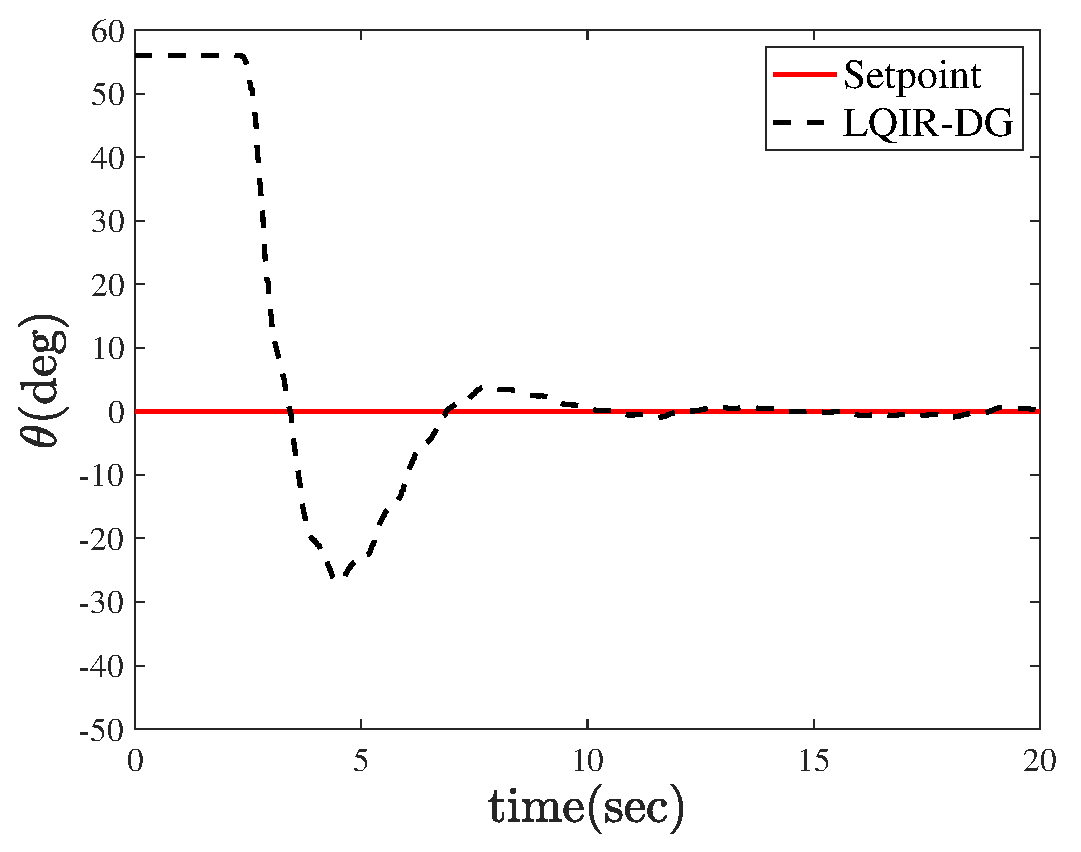
\includegraphics[width=.49\linewidth]{../Figure/implementation/lqidg_pitch}
	}
	\hfil
	\subfloat[]{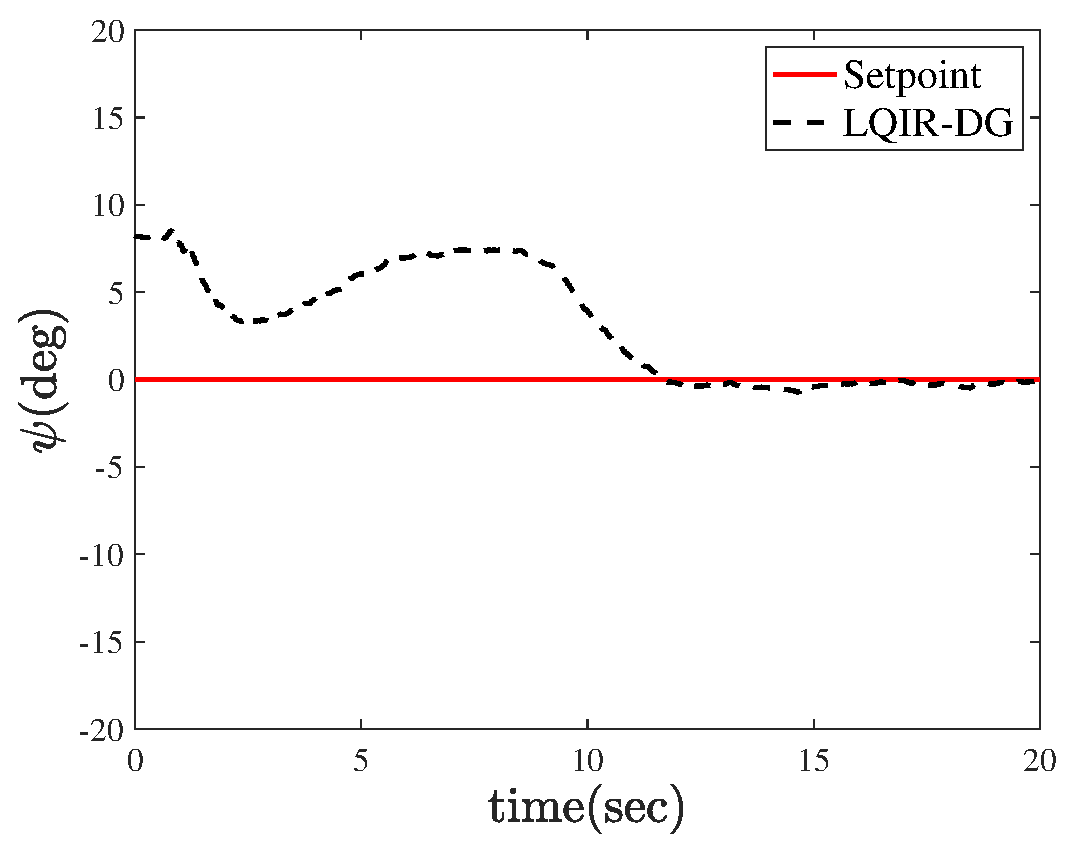
\includegraphics[width=.49\linewidth]{../Figure/implementation/lqidg_yaw}\label{fig:pitch}
	}
	\caption{Performance of the LQIR-DG controller (a) roll angle (b) pitch angle (c) yaw angle}
	\label{fig:result}
\end{figure}

\begin{figure}[!h]
	\centering
	\subfloat[]{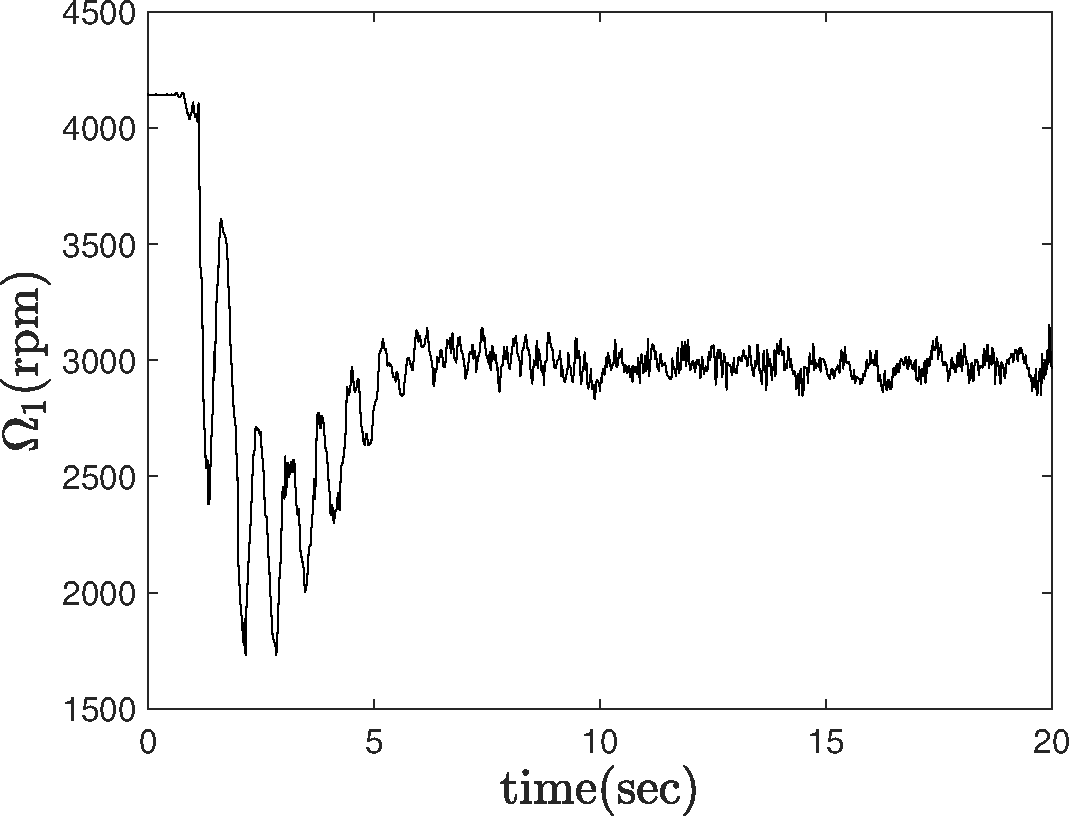
\includegraphics[width=.49\linewidth]{../Figure/implementation/lqidg_Omega_1}}\subfloat[]{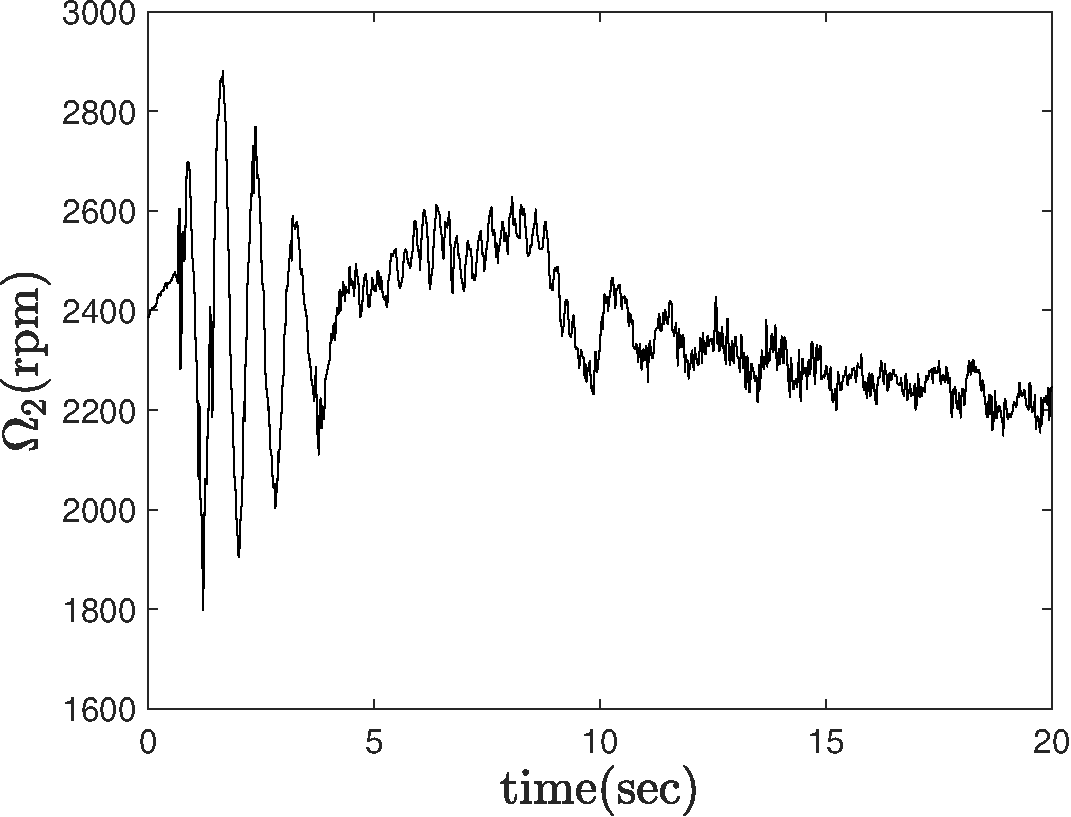
\includegraphics[width=.49\linewidth]{../Figure/implementation/lqidg_Omega_2}
	}
	\hfil
	\subfloat[]{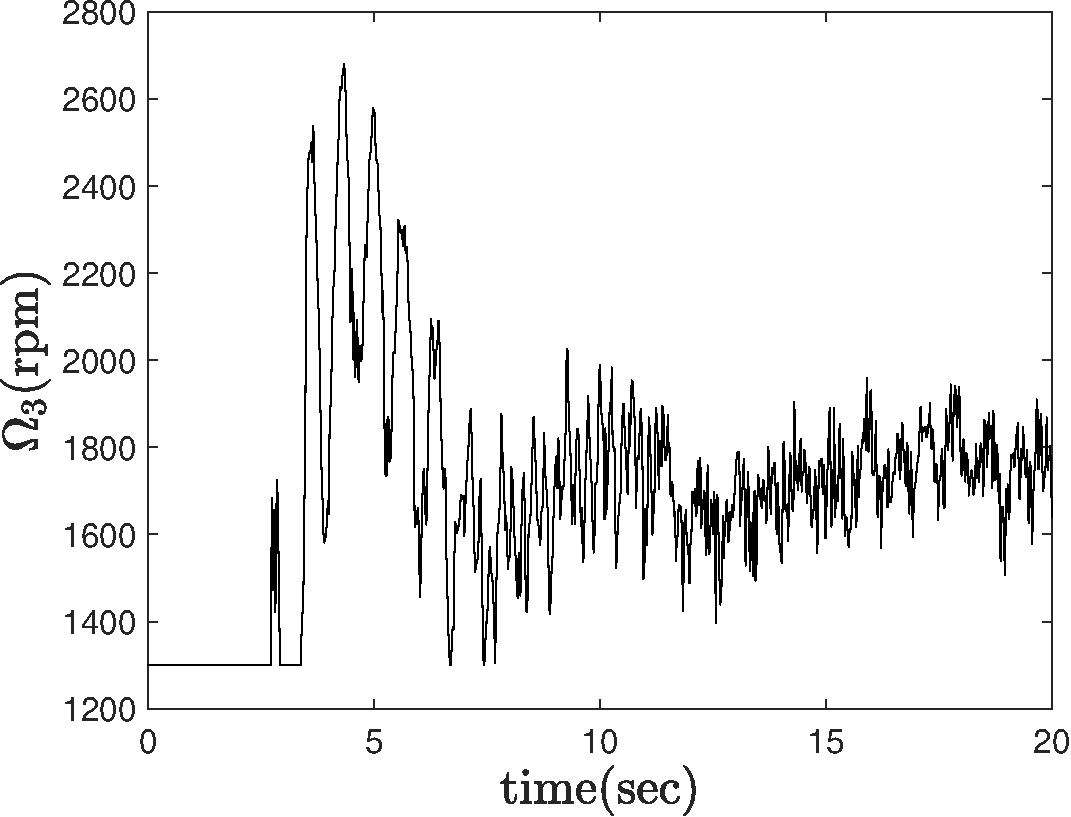
\includegraphics[width=.49\linewidth]{../Figure/implementation/lqidg_Omega_3}}\subfloat[]{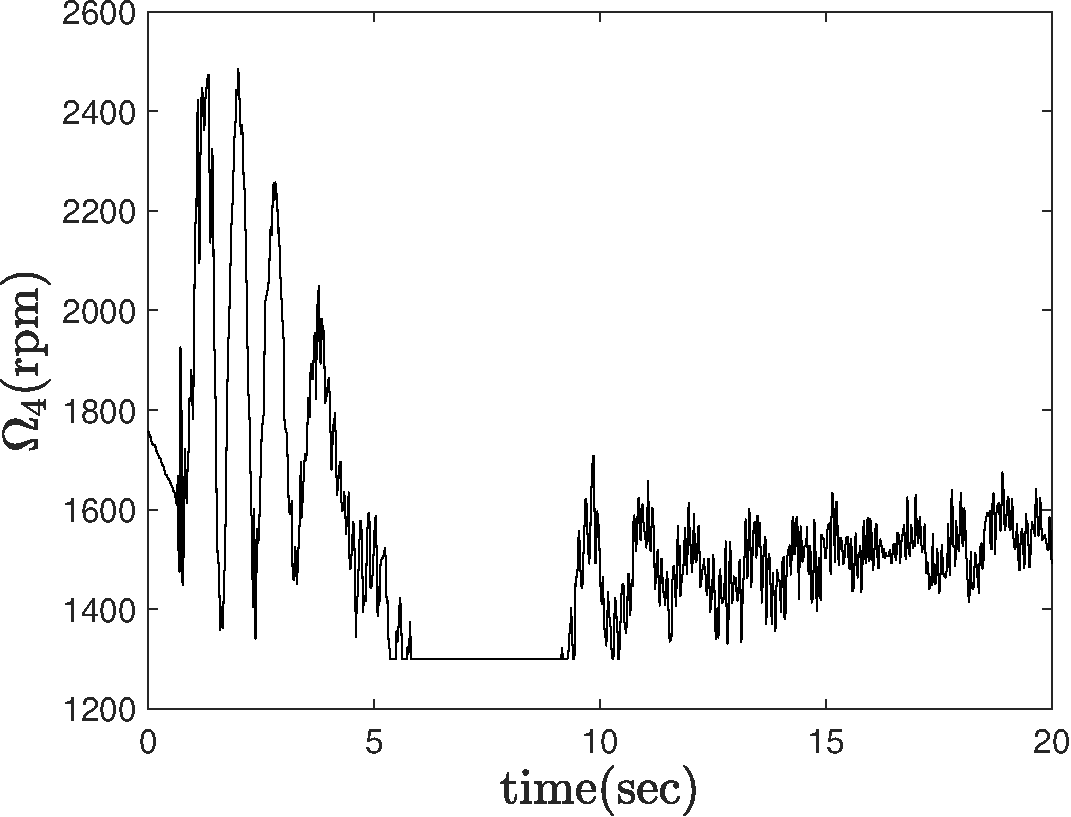
\includegraphics[width=.49\linewidth]{../Figure/implementation/lqidg_Omega_4}
	}
	\caption{Time history of angular velocity commands}
	\label{fig:omega}
\end{figure}


Figure \ref{fig:square} illustrates the performance of the LQIR-DG controller in the coupling mode of the roll and pitch channels to track the desired angle as a square wave with a frequency of 0.02 Hz and an amplitude of 20 degrees.

\begin{figure}[!ht]
	\centering
	\subfloat[]{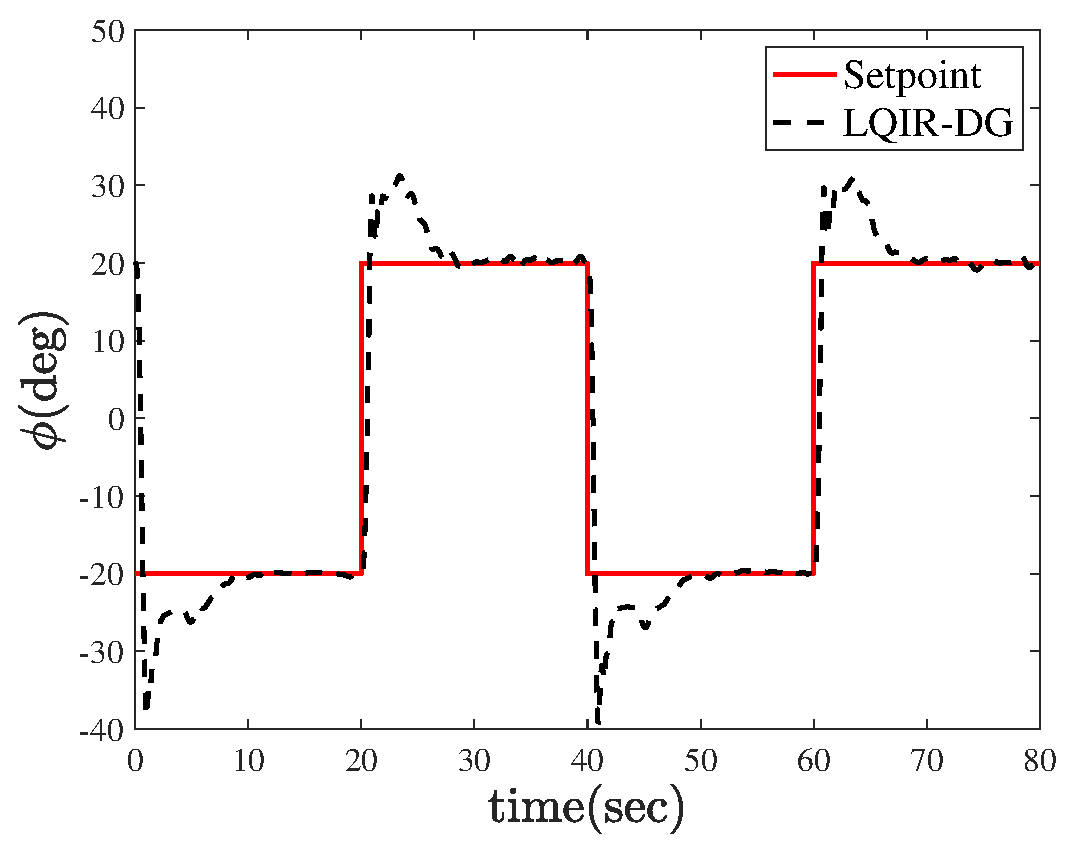
\includegraphics[width=.49\linewidth]{../Figure/implementation/square/lqidg_roll_20}}\subfloat[]{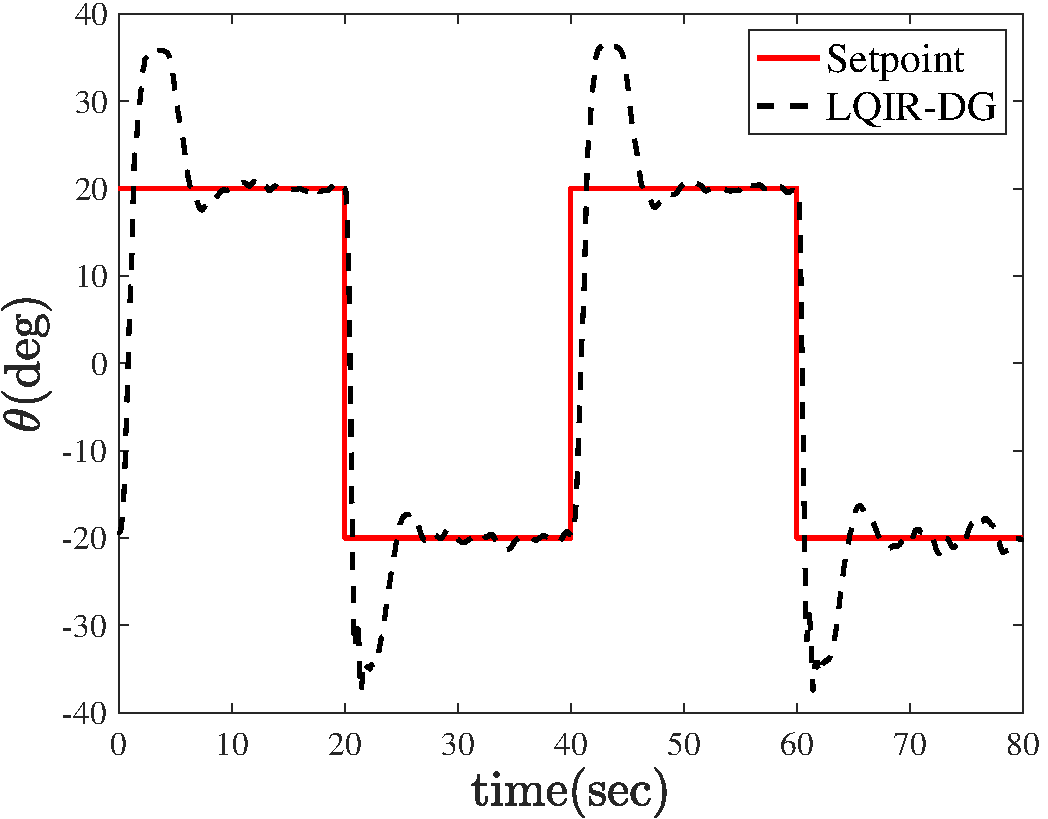
\includegraphics[width=.49\linewidth]{../Figure/implementation/square/lqidg_pitch_20}
	}
	\caption{LQIR-DDG controller performance in order to track the desired angles in the two-degree-of-freedom coupling mode (a) Comparison of the roll angle with the desired value (b) Comparison of the pitch angle with the desired}
	\label{fig:square}
\end{figure}

\subsection{Investigating the possibility of disturbance rejection}

\noindent This section investigates the possible rejection of input disturbances by the LQIR-DG controller in regulation. For this purpose, a disturbance with an amplitude of 0.5 N is added to the input from 20 to 60 seconds. As shown in figure \ref{fig:disturbance}, the LQIR-DG controller performs well in coupling the roll and screw channels to remove the input disturbance. \ref{fig:disturbance} (a), the performance of this controller is checked by comparing the desired roll angle with the actual roll angle. Also, \ref{fig:disturbance}  (b) compares the desired pitch angle with the actual pitch angle of the 3DoF experimental setup in removing the input disturbance. The results indicate the proper performance of the controller in removing the input disturbance.

\begin{figure}[!ht]
	\centering
	\subfloat[]{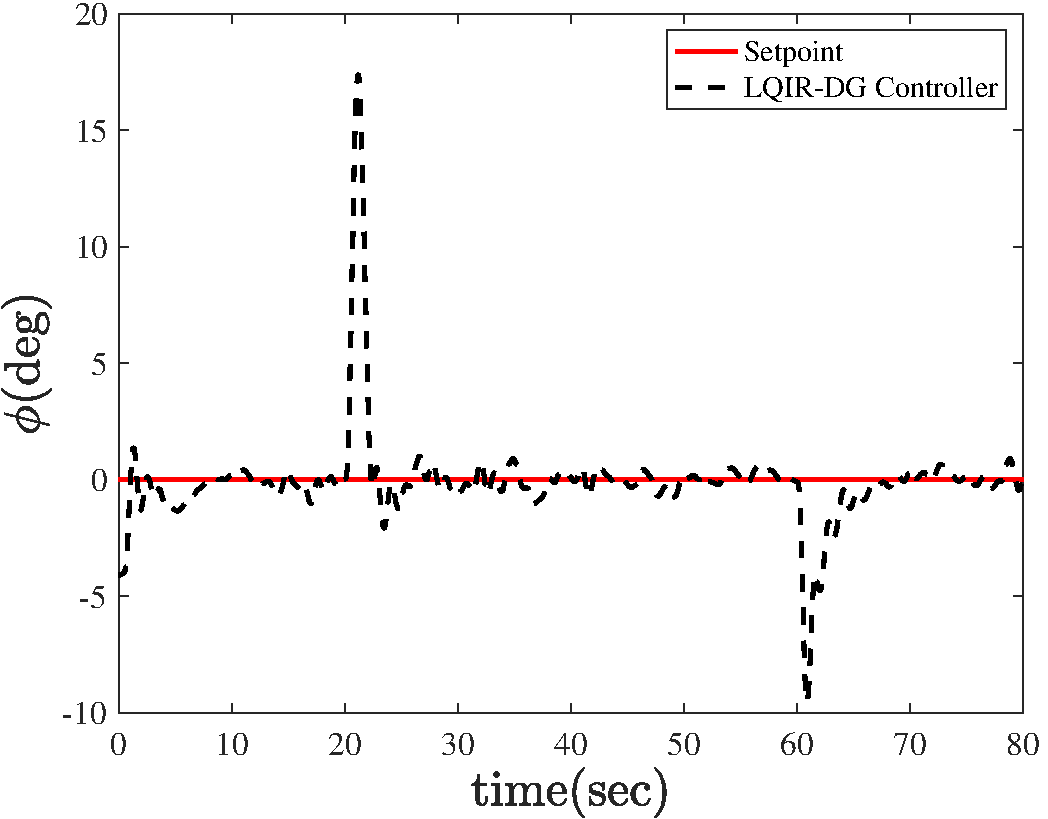
\includegraphics[width=.49\linewidth]{../Figure/implementation/disturbance/lqidg_roll}}\subfloat[]{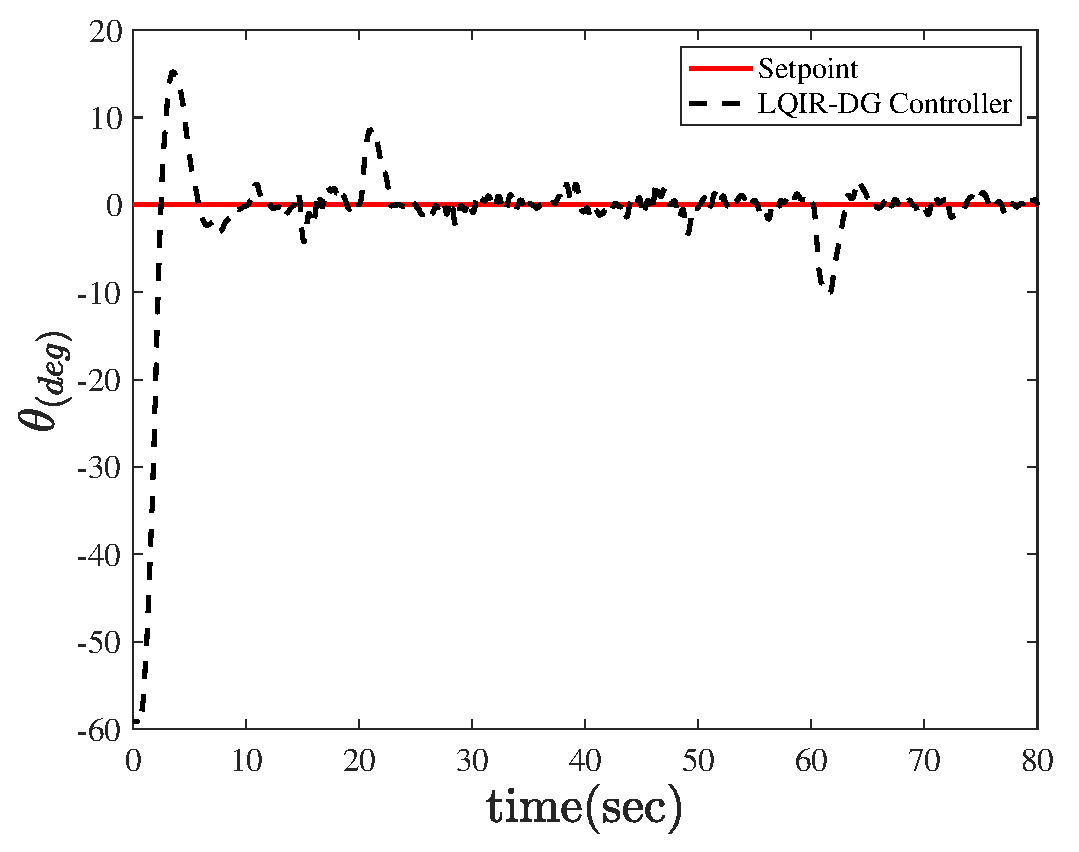
\includegraphics[width=.49\linewidth]{../Figure/implementation/disturbance/lqidg_pitch}
	}
	\caption{The performance of the LQIR-DG controller in the presence of the input disturbance in the two-degree-of-freedom coupling mode (a) Comparison of the desired roll angle with the actual value (b) Comparison of the desired pitch angle with the actual value.}
	\label{fig:disturbance}
\end{figure}

\subsection{Investigating the impact of uncertainty in modeling }
\noindent This section examines the performance of the LQIR-DG controller designed by considering the uncertainty in 3DoF experimental setup modeling. The performance of the sliding mode con-troller in the coupling mode of the roll, pitch, and yaw channels is checked by considering the uncertainty in the 3DoF experimental setup modeling in figure \ref{fig:weight}. For this purpose, 50 grams is added to the roll axis and 100 grams to the pitch axis. In figure \ref{fig:weight} (a), the performance of this con-troller is checked by comparing the desired roll angle with the actual roll angle; In figure \ref{fig:weight} (b), the performance of this controller is checked by comparing the desired pitch angle to the actual pitch angle. Also, figure \ref{fig:weight} (c) compares the desired yaw angle with the actual yaw angle of the 3DoF experimental setup. The implementation results indicate the proper efficiency of the LQIR-DG controller in pursuit of the desired value, taking into account the uncertainty in the values of the moments of inertia around each axis of the body coordinate system.
\begin{figure}[!h]
	\centering
	\subfloat[]{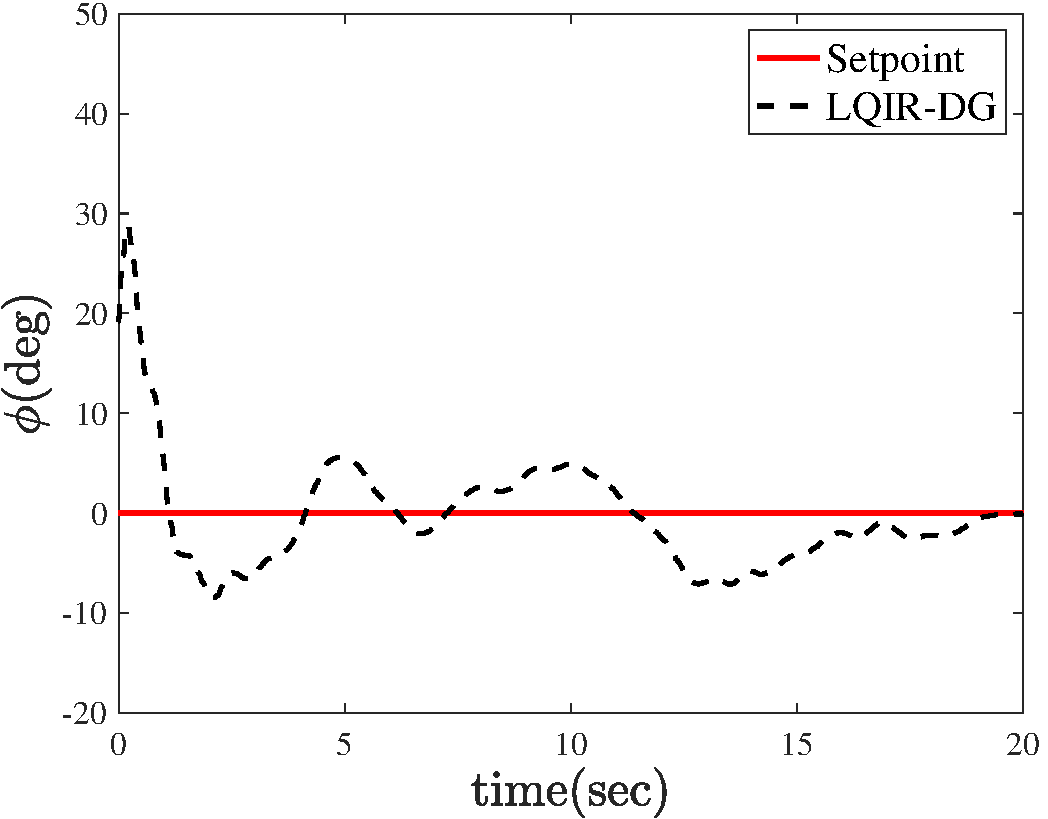
\includegraphics[width=.49\linewidth]{../Figure/implementation/weight/lqidg_roll}}\subfloat[]{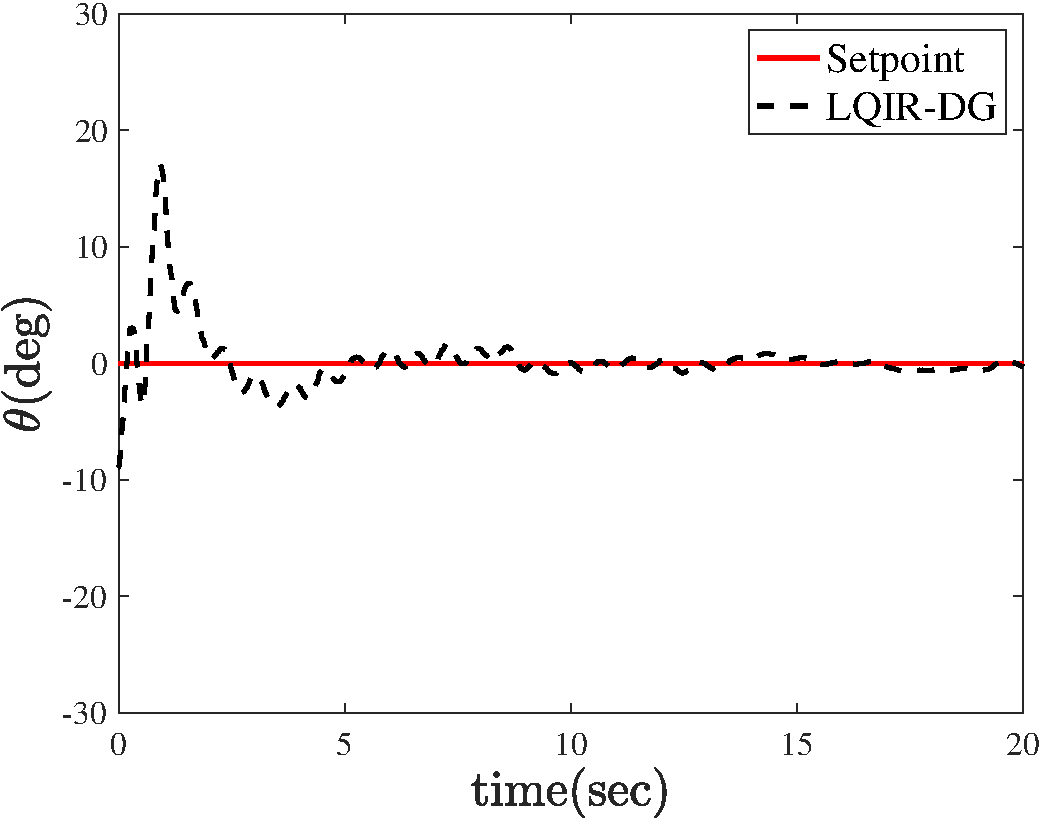
\includegraphics[width=.49\linewidth]{../Figure/implementation/weight/lqidg_pitch}
	}
	\hfil
	\subfloat[]{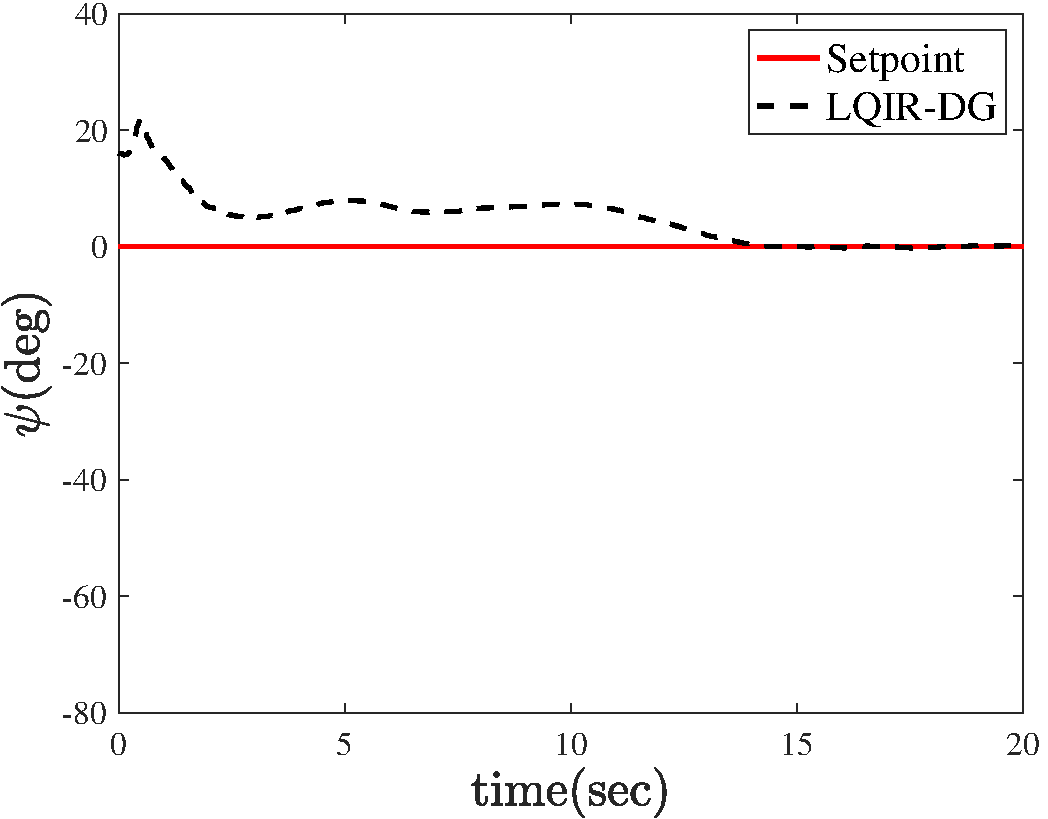
\includegraphics[width=.49\linewidth]{../Figure/implementation/weight/lqidg_yaw}
	}
	\caption{The performance of the LQIR-DG controller by adding weight to each of the roll and pitch axes in the three-degree-of-freedom coupling mode (a) Comparison of the roll angle with the actual value (b) Comparison of the pitch angle with the actual value (c) Comparison of the yaw angle with the actual value}
	\label{fig:weight}
\end{figure}

\subsection{Comparison with LQR}
\noindent Here, the LQIR-DG controller performance is compared with famous control strategies such as the LQR controller method. \figurename{\ref{fig:compare}} compares the quadrotor's desired and actual pitch angle in the presence of these controllers. This result indicates that the LQIR-DG controller can provide high tracking performance, such as good transient response and high rapid convergence relative to the LQR controller for pitch angle control of the quadrotor setup.
\begin{figure}[!h]
	\centering
	{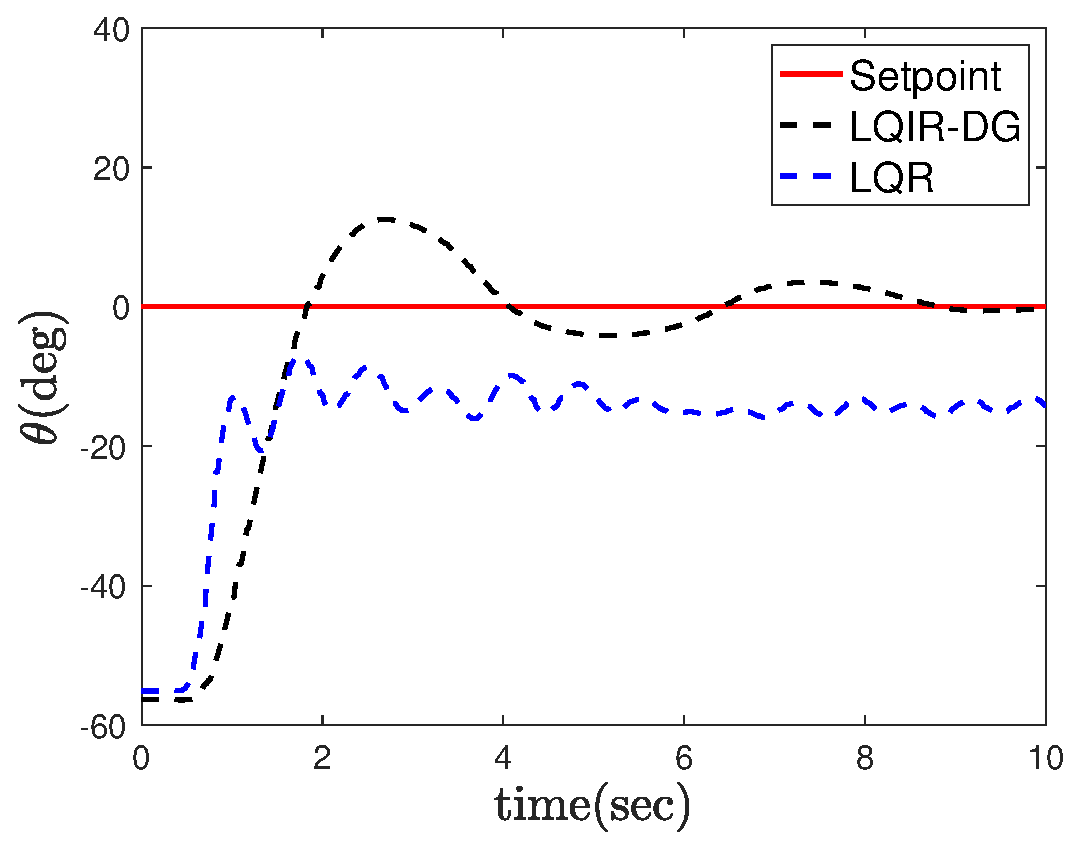
\includegraphics[width=.49\linewidth]{../Figure/implementation/lqidgvslqr/lqidgvslqr_pitch}
	}
	\caption{Comparison of the LQIR-DG to the LQR in control of the pitch angle of the experimental setup}
	\label{fig:compare}
\end{figure}

\begin{figure}[!h]
	\centering
	{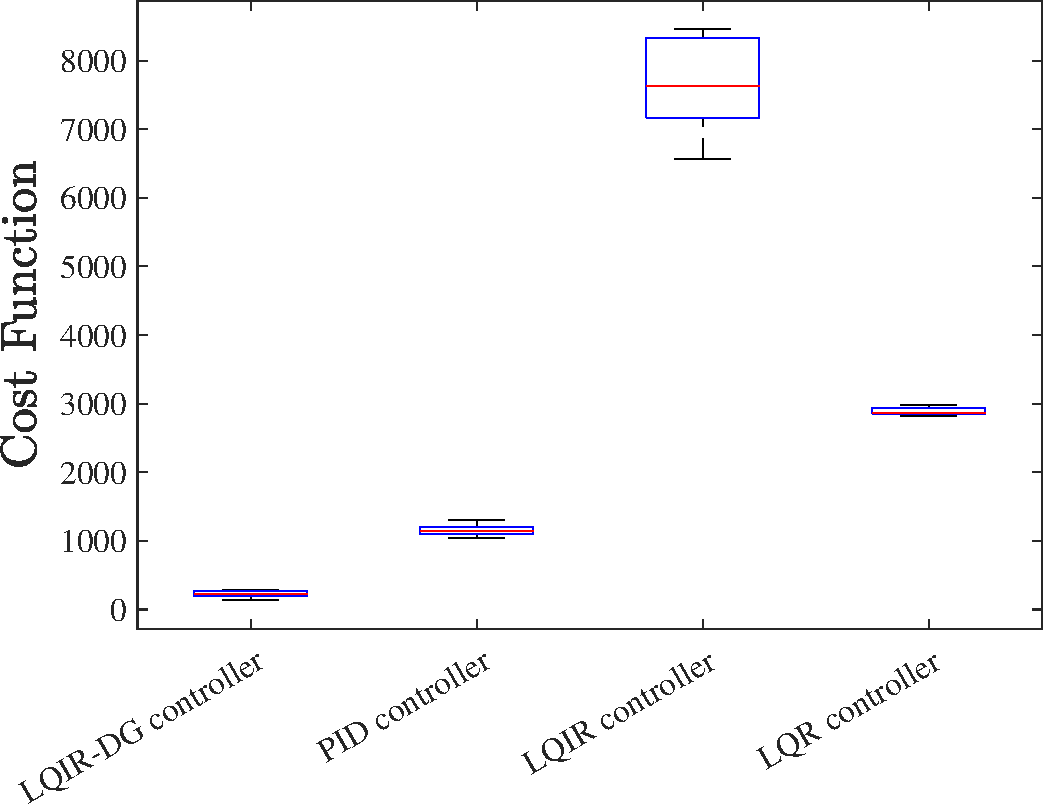
\includegraphics[width=.49\linewidth]{../Figure/implementation/box_plot/lqidgvsboxplot}
	}
	\caption{Comparison of the LQIR-DG to the PID quadratic cost function}
	\label{fig:compare_boxplot}
\end{figure}


\section{Conclusion}\label{sec:conclusion}
\noindent In this study, a linear quadratic with integral action based on the differential game theory, called LQIR-DG, was implemented for level attitude control in an experimental setup of a quadrotor. To implement the proposed controller structure, first, an accurate model of the quadrotor was linearized in the state-space form, and then the model parameters were estimated. Next, two players were considered for each of the quadrotor's roll, pitch, and yaw channels. The first player found the best control command for each channel of the setup of a quadrotor based on the mini-maximization of a quadratic criterion; when the second player produced the worst disturbances. Finally, the performance of the proposed controller was investigated in level flight and compared to the LQR controller. The implementation results verify the successful performance of the LQIR-DG method in the level flight of the attitude control for the actual plant.





%% The Appendices part is started with the command \appendix;
%% appendix sections are then done as normal sections
%% \appendix

%% \section{}
%% \label{}

%% References
%%
%% Following citation commands can be used in the body text:
%% Usage of \cite is as follows:
%%   \cite{key}         ==>>  [#]
%%   \cite[chap. 2]{key} ==>> [#, chap. 2]
%%

%% References with BibTeX database:

\bibliographystyle{elsarticle-num}
\bibliography{refs}

%% Authors are advised to use a BibTeX database file for their reference list.
%% The provided style file elsarticle-num.bst formats references in the required Procedia style

%% For references without a BibTeX database:

% \begin{thebibliography}{00}

%% \bibitem must have the following form:
%%   \bibitem{key}...
%%

% \bibitem{}

% \end{thebibliography}


\end{document}

%%
%% End of file `ecrc-template.tex'. 